\section{Data Mining}
\label{sec:data_mining}

This section describes the experiments that were performed on the datasets to obtain a better understanding of what makes a good recipe.
First, the itemsets of ingredients are mined for general patterns using association rule mining.
After that, the dataset is divided into two clusters, a positive and negative dataset, using the rating dataset.
A decision tree model is then used to learn a decision boundary between these two clusters, which is then analyzed in detail.


%============================================================


\subsection{Association Rule Mining}
\label{subsec:association_rule_mining}

This section covers the analysis of the ingredient dataset using association rule mining.
Using the apriori algorithm, we mine the dataset for association rules with a confidence of $0.5$ and a coverage of $0.02$, resulting in a set of $1003$ association rules.
\cref{tab:rules_top10} shows the association rules that have the highest lift.
They describe patterns commonly found in sweet, oven-baked dishes, such as cookies and pies.
Nutmeg and cinnamon are often used in combination with clover in cookie mixes (e.g. in `speculaas'), so it is not strange to find the pattern \{nutmeg\} $\rightarrow$ \{cinnamon\}.
The list is however dominated by vanilla as the antecedent and very similar rules.
This could be caused by a strong bias towards these type of dishes in the dataset, because this would result in a high coverage, which is one of the interestingness measures the rules are pruned on.
Looking more closely at the recipes, this does not seem the case, however, as depicted before in \cref{fig:ingredient_frequencies}.
Many recipes include ingredients such as pepper, onions and cheese, which are normally not used in deserts.
This result shows that the ingredients used in these meals are more predictable, in that they are often used in a similar way.


\begin{table}[htbp]
	\caption{Top 10 of association rules ordered by lift.}
	\label{tab:rules_top10}
	
	\centering
	\begin{tabular}{l l l l}
		\toprule
		\textbf{Rule} & \textbf{Sup.} & \textbf{Conf.} & \textbf{Lift} \\
		\midrule
		\{nutmeg\} $\rightarrow$ \{cinnamon\} & 0.024 & 0.58 & 6.23 \\
		\{chocolate, eggs, sugar\} $\rightarrow$ \{vanilla\} & 0.024 & 0.68 & 5.04 \\
		\{chocolate, flour, sugar\} $\rightarrow$ \{vanilla\} & 0.020 & 0.68 & 5.00 \\
		\{chocolate, flour\} $\rightarrow$ \{vanilla\} & 0.021 & 0.67 & 4.94 \\
		\{chocolate, salt\} $\rightarrow$ \{vanilla\} & 0.020 & 0.66 & 4.89 \\
		\{chocolate, eggs\} $\rightarrow$ \{vanilla\} & 0.025 & 0.64 & 4.76 \\
		\{butter, eggs, flour, salt, sugar\} $\rightarrow$ \{vanilla\} & 0.029 & 0.61 & 4.54 \\
		\{butter, eggs, flour, sugar\} $\rightarrow$ \{vanilla\} & 0.042 & 0.61 & 4.51 \\
		\{butter, eggs, salt, sugar\} $\rightarrow$ \{vanilla\} & 0.031 & 0.61 & 4.49 \\
		\{butter, eggs, milk, sugar\} $\rightarrow$ \{vanilla\} & 0.022 & 0.60 & 4.45 \\
		\bottomrule
	\end{tabular}
	
\end{table}

\begin{figure}[htbp]
	% Created by tikzDevice version 0.10.1 on 2016-07-27 18:04:24
% !TEX encoding = UTF-8 Unicode
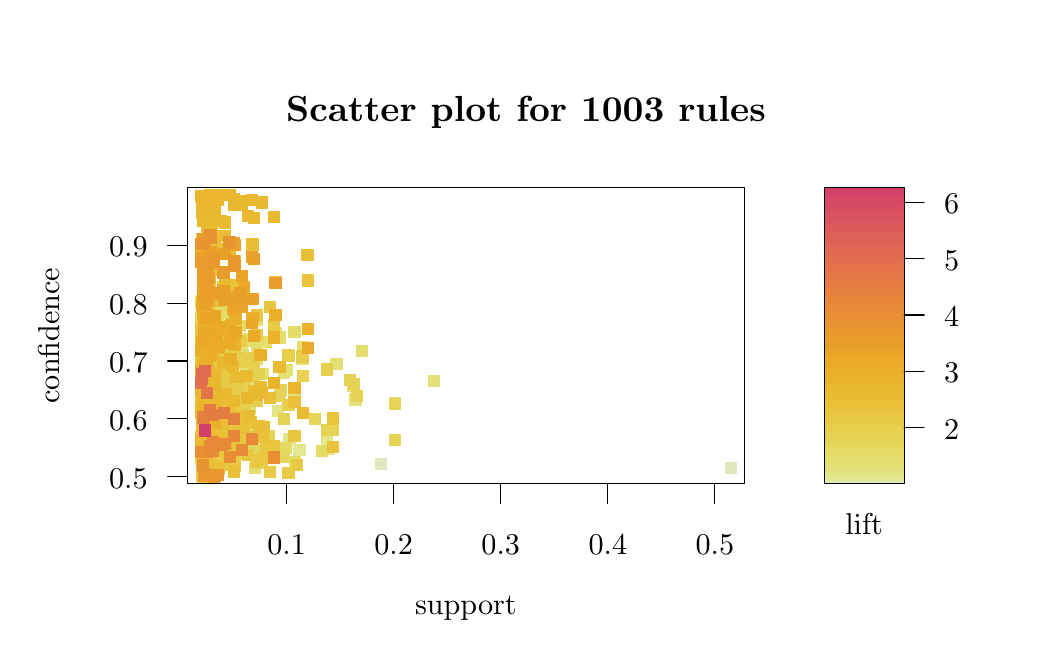
\begin{tikzpicture}[x=1pt,y=1pt]
\definecolor{fillColor}{RGB}{255,255,255}
\path[use as bounding box,fill=fillColor,fill opacity=0.00] (0,0) rectangle (360.07,222.54);
\begin{scope}
\path[clip] (  0.00,  0.00) rectangle (360.07,222.54);
\definecolor{drawColor}{RGB}{0,0,0}

\node[text=drawColor,anchor=base,inner sep=0pt, outer sep=0pt, scale=  1.31] at (180.04,188.69) {\bfseries Scatter plot for 1003 rules};
\end{scope}
\begin{scope}
\path[clip] (  0.00,  0.00) rectangle (360.07,222.54);
\definecolor{fillColor}{RGB}{226,230,189}

\path[fill=fillColor] (287.80, 57.82) rectangle (316.71, 58.89);
\definecolor{fillColor}{RGB}{226,231,145}

\path[fill=fillColor] (287.80, 58.89) rectangle (316.71, 59.95);
\definecolor{fillColor}{RGB}{226,230,136}

\path[fill=fillColor] (287.80, 59.95) rectangle (316.71, 61.02);
\definecolor{fillColor}{RGB}{226,229,130}

\path[fill=fillColor] (287.80, 61.02) rectangle (316.71, 62.09);
\definecolor{fillColor}{RGB}{226,227,125}

\path[fill=fillColor] (287.80, 62.09) rectangle (316.71, 63.16);
\definecolor{fillColor}{RGB}{227,226,120}

\path[fill=fillColor] (287.80, 63.16) rectangle (316.71, 64.23);
\definecolor{fillColor}{RGB}{227,225,115}

\path[fill=fillColor] (287.80, 64.23) rectangle (316.71, 65.30);
\definecolor{fillColor}{RGB}{227,223,111}

\path[fill=fillColor] (287.80, 65.30) rectangle (316.71, 66.37);
\definecolor{fillColor}{RGB}{228,222,108}

\path[fill=fillColor] (287.80, 66.37) rectangle (316.71, 67.44);
\definecolor{fillColor}{RGB}{228,220,104}

\path[fill=fillColor] (287.80, 67.44) rectangle (316.71, 68.51);
\definecolor{fillColor}{RGB}{228,219,100}

\path[fill=fillColor] (287.80, 68.51) rectangle (316.71, 69.58);
\definecolor{fillColor}{RGB}{229,217,97}

\path[fill=fillColor] (287.80, 69.58) rectangle (316.71, 70.65);
\definecolor{fillColor}{RGB}{229,216,94}

\path[fill=fillColor] (287.80, 70.65) rectangle (316.71, 71.71);
\definecolor{fillColor}{RGB}{229,214,91}

\path[fill=fillColor] (287.80, 71.71) rectangle (316.71, 72.78);
\definecolor{fillColor}{RGB}{229,212,88}

\path[fill=fillColor] (287.80, 72.78) rectangle (316.71, 73.85);
\definecolor{fillColor}{RGB}{230,211,85}

\path[fill=fillColor] (287.80, 73.85) rectangle (316.71, 74.92);
\definecolor{fillColor}{RGB}{230,209,82}

\path[fill=fillColor] (287.80, 74.92) rectangle (316.71, 75.99);
\definecolor{fillColor}{RGB}{230,208,79}

\path[fill=fillColor] (287.80, 75.99) rectangle (316.71, 77.06);
\definecolor{fillColor}{RGB}{231,206,76}

\path[fill=fillColor] (287.80, 77.06) rectangle (316.71, 78.13);
\definecolor{fillColor}{RGB}{231,205,74}

\path[fill=fillColor] (287.80, 78.13) rectangle (316.71, 79.20);
\definecolor{fillColor}{RGB}{231,203,71}

\path[fill=fillColor] (287.80, 79.20) rectangle (316.71, 80.27);
\definecolor{fillColor}{RGB}{231,201,68}

\path[fill=fillColor] (287.80, 80.27) rectangle (316.71, 81.34);
\definecolor{fillColor}{RGB}{232,200,66}

\path[fill=fillColor] (287.80, 81.34) rectangle (316.71, 82.40);
\definecolor{fillColor}{RGB}{232,198,64}

\path[fill=fillColor] (287.80, 82.40) rectangle (316.71, 83.47);
\definecolor{fillColor}{RGB}{232,197,61}

\path[fill=fillColor] (287.80, 83.47) rectangle (316.71, 84.54);
\definecolor{fillColor}{RGB}{232,195,59}

\path[fill=fillColor] (287.80, 84.54) rectangle (316.71, 85.61);
\definecolor{fillColor}{RGB}{232,193,57}

\path[fill=fillColor] (287.80, 85.61) rectangle (316.71, 86.68);
\definecolor{fillColor}{RGB}{233,192,55}

\path[fill=fillColor] (287.80, 86.68) rectangle (316.71, 87.75);
\definecolor{fillColor}{RGB}{233,190,53}

\path[fill=fillColor] (287.80, 87.75) rectangle (316.71, 88.82);
\definecolor{fillColor}{RGB}{233,188,51}

\path[fill=fillColor] (287.80, 88.82) rectangle (316.71, 89.89);
\definecolor{fillColor}{RGB}{233,187,50}

\path[fill=fillColor] (287.80, 89.89) rectangle (316.71, 90.96);
\definecolor{fillColor}{RGB}{233,185,48}

\path[fill=fillColor] (287.80, 90.96) rectangle (316.71, 92.03);
\definecolor{fillColor}{RGB}{233,184,47}

\path[fill=fillColor] (287.80, 92.03) rectangle (316.71, 93.10);
\definecolor{fillColor}{RGB}{233,182,45}

\path[fill=fillColor] (287.80, 93.10) rectangle (316.71, 94.16);
\definecolor{fillColor}{RGB}{233,180,44}

\path[fill=fillColor] (287.80, 94.16) rectangle (316.71, 95.23);
\definecolor{fillColor}{RGB}{234,179,43}

\path[fill=fillColor] (287.80, 95.23) rectangle (316.71, 96.30);
\definecolor{fillColor}{RGB}{234,177,42}

\path[fill=fillColor] (287.80, 96.30) rectangle (316.71, 97.37);
\definecolor{fillColor}{RGB}{234,175,41}

\path[fill=fillColor] (287.80, 97.37) rectangle (316.71, 98.44);
\definecolor{fillColor}{RGB}{234,174,41}

\path[fill=fillColor] (287.80, 98.44) rectangle (316.71, 99.51);
\definecolor{fillColor}{RGB}{234,172,40}

\path[fill=fillColor] (287.80, 99.51) rectangle (316.71,100.58);
\definecolor{fillColor}{RGB}{234,170,40}

\path[fill=fillColor] (287.80,100.58) rectangle (316.71,101.65);
\definecolor{fillColor}{RGB}{234,169,40}

\path[fill=fillColor] (287.80,101.65) rectangle (316.71,102.72);
\definecolor{fillColor}{RGB}{234,167,40}

\path[fill=fillColor] (287.80,102.72) rectangle (316.71,103.79);
\definecolor{fillColor}{RGB}{234,165,40}

\path[fill=fillColor] (287.80,103.79) rectangle (316.71,104.86);
\definecolor{fillColor}{RGB}{234,164,40}

\path[fill=fillColor] (287.80,104.86) rectangle (316.71,105.92);
\definecolor{fillColor}{RGB}{233,162,41}

\path[fill=fillColor] (287.80,105.92) rectangle (316.71,106.99);
\definecolor{fillColor}{RGB}{233,160,41}

\path[fill=fillColor] (287.80,106.99) rectangle (316.71,108.06);
\definecolor{fillColor}{RGB}{233,159,42}

\path[fill=fillColor] (287.80,108.06) rectangle (316.71,109.13);
\definecolor{fillColor}{RGB}{233,157,43}

\path[fill=fillColor] (287.80,109.13) rectangle (316.71,110.20);
\definecolor{fillColor}{RGB}{233,155,43}

\path[fill=fillColor] (287.80,110.20) rectangle (316.71,111.27);
\definecolor{fillColor}{RGB}{233,154,44}

\path[fill=fillColor] (287.80,111.27) rectangle (316.71,112.34);
\definecolor{fillColor}{RGB}{233,152,45}

\path[fill=fillColor] (287.80,112.34) rectangle (316.71,113.41);
\definecolor{fillColor}{RGB}{233,150,46}

\path[fill=fillColor] (287.80,113.41) rectangle (316.71,114.48);
\definecolor{fillColor}{RGB}{232,148,48}

\path[fill=fillColor] (287.80,114.48) rectangle (316.71,115.55);
\definecolor{fillColor}{RGB}{232,147,49}

\path[fill=fillColor] (287.80,115.55) rectangle (316.71,116.62);
\definecolor{fillColor}{RGB}{232,145,50}

\path[fill=fillColor] (287.80,116.62) rectangle (316.71,117.68);
\definecolor{fillColor}{RGB}{232,143,51}

\path[fill=fillColor] (287.80,117.68) rectangle (316.71,118.75);
\definecolor{fillColor}{RGB}{232,142,53}

\path[fill=fillColor] (287.80,118.75) rectangle (316.71,119.82);
\definecolor{fillColor}{RGB}{231,140,54}

\path[fill=fillColor] (287.80,119.82) rectangle (316.71,120.89);
\definecolor{fillColor}{RGB}{231,138,55}

\path[fill=fillColor] (287.80,120.89) rectangle (316.71,121.96);
\definecolor{fillColor}{RGB}{231,137,57}

\path[fill=fillColor] (287.80,121.96) rectangle (316.71,123.03);
\definecolor{fillColor}{RGB}{230,135,58}

\path[fill=fillColor] (287.80,123.03) rectangle (316.71,124.10);
\definecolor{fillColor}{RGB}{230,133,59}

\path[fill=fillColor] (287.80,124.10) rectangle (316.71,125.17);
\definecolor{fillColor}{RGB}{230,131,61}

\path[fill=fillColor] (287.80,125.17) rectangle (316.71,126.24);
\definecolor{fillColor}{RGB}{230,130,62}

\path[fill=fillColor] (287.80,126.24) rectangle (316.71,127.31);
\definecolor{fillColor}{RGB}{229,128,64}

\path[fill=fillColor] (287.80,127.31) rectangle (316.71,128.38);
\definecolor{fillColor}{RGB}{229,126,65}

\path[fill=fillColor] (287.80,128.38) rectangle (316.71,129.44);
\definecolor{fillColor}{RGB}{228,124,66}

\path[fill=fillColor] (287.80,129.44) rectangle (316.71,130.51);
\definecolor{fillColor}{RGB}{228,123,68}

\path[fill=fillColor] (287.80,130.51) rectangle (316.71,131.58);
\definecolor{fillColor}{RGB}{228,121,69}

\path[fill=fillColor] (287.80,131.58) rectangle (316.71,132.65);
\definecolor{fillColor}{RGB}{227,119,71}

\path[fill=fillColor] (287.80,132.65) rectangle (316.71,133.72);
\definecolor{fillColor}{RGB}{227,117,72}

\path[fill=fillColor] (287.80,133.72) rectangle (316.71,134.79);
\definecolor{fillColor}{RGB}{226,116,73}

\path[fill=fillColor] (287.80,134.79) rectangle (316.71,135.86);
\definecolor{fillColor}{RGB}{226,114,75}

\path[fill=fillColor] (287.80,135.86) rectangle (316.71,136.93);
\definecolor{fillColor}{RGB}{226,112,76}

\path[fill=fillColor] (287.80,136.93) rectangle (316.71,138.00);
\definecolor{fillColor}{RGB}{225,110,77}

\path[fill=fillColor] (287.80,138.00) rectangle (316.71,139.07);
\definecolor{fillColor}{RGB}{225,109,79}

\path[fill=fillColor] (287.80,139.07) rectangle (316.71,140.14);
\definecolor{fillColor}{RGB}{224,107,80}

\path[fill=fillColor] (287.80,140.14) rectangle (316.71,141.20);
\definecolor{fillColor}{RGB}{224,105,81}

\path[fill=fillColor] (287.80,141.20) rectangle (316.71,142.27);
\definecolor{fillColor}{RGB}{223,103,83}

\path[fill=fillColor] (287.80,142.27) rectangle (316.71,143.34);
\definecolor{fillColor}{RGB}{223,101,84}

\path[fill=fillColor] (287.80,143.34) rectangle (316.71,144.41);
\definecolor{fillColor}{RGB}{222,99,85}

\path[fill=fillColor] (287.80,144.41) rectangle (316.71,145.48);
\definecolor{fillColor}{RGB}{221,98,86}

\path[fill=fillColor] (287.80,145.48) rectangle (316.71,146.55);
\definecolor{fillColor}{RGB}{221,96,88}

\path[fill=fillColor] (287.80,146.55) rectangle (316.71,147.62);
\definecolor{fillColor}{RGB}{220,94,89}

\path[fill=fillColor] (287.80,147.62) rectangle (316.71,148.69);
\definecolor{fillColor}{RGB}{220,92,90}

\path[fill=fillColor] (287.80,148.69) rectangle (316.71,149.76);
\definecolor{fillColor}{RGB}{219,90,91}

\path[fill=fillColor] (287.80,149.76) rectangle (316.71,150.83);
\definecolor{fillColor}{RGB}{219,88,93}

\path[fill=fillColor] (287.80,150.83) rectangle (316.71,151.90);
\definecolor{fillColor}{RGB}{218,86,94}

\path[fill=fillColor] (287.80,151.90) rectangle (316.71,152.96);
\definecolor{fillColor}{RGB}{217,84,95}

\path[fill=fillColor] (287.80,152.96) rectangle (316.71,154.03);
\definecolor{fillColor}{RGB}{217,82,96}

\path[fill=fillColor] (287.80,154.03) rectangle (316.71,155.10);
\definecolor{fillColor}{RGB}{216,80,97}

\path[fill=fillColor] (287.80,155.10) rectangle (316.71,156.17);
\definecolor{fillColor}{RGB}{215,78,98}

\path[fill=fillColor] (287.80,156.17) rectangle (316.71,157.24);
\definecolor{fillColor}{RGB}{215,76,99}

\path[fill=fillColor] (287.80,157.24) rectangle (316.71,158.31);
\definecolor{fillColor}{RGB}{214,74,101}

\path[fill=fillColor] (287.80,158.31) rectangle (316.71,159.38);
\definecolor{fillColor}{RGB}{213,72,102}

\path[fill=fillColor] (287.80,159.38) rectangle (316.71,160.45);
\definecolor{fillColor}{RGB}{213,70,103}

\path[fill=fillColor] (287.80,160.45) rectangle (316.71,161.52);
\definecolor{fillColor}{RGB}{212,68,104}

\path[fill=fillColor] (287.80,161.52) rectangle (316.71,162.59);
\definecolor{fillColor}{RGB}{211,66,105}

\path[fill=fillColor] (287.80,162.59) rectangle (316.71,163.66);
\definecolor{fillColor}{RGB}{211,63,106}

\path[fill=fillColor] (287.80,163.66) rectangle (316.71,164.72);
\definecolor{drawColor}{RGB}{0,0,0}

\path[draw=drawColor,line width= 0.4pt,line join=round,line cap=round] (287.80, 57.82) rectangle (316.71,164.72);

\path[draw=drawColor,line width= 0.4pt,line join=round,line cap=round] (316.71, 78.00) --
	(316.71,159.41);

\path[draw=drawColor,line width= 0.4pt,line join=round,line cap=round] (316.71, 78.00) -- (323.94, 78.00);

\path[draw=drawColor,line width= 0.4pt,line join=round,line cap=round] (316.71, 98.35) -- (323.94, 98.35);

\path[draw=drawColor,line width= 0.4pt,line join=round,line cap=round] (316.71,118.70) -- (323.94,118.70);

\path[draw=drawColor,line width= 0.4pt,line join=round,line cap=round] (316.71,139.06) -- (323.94,139.06);

\path[draw=drawColor,line width= 0.4pt,line join=round,line cap=round] (316.71,159.41) -- (323.94,159.41);

\node[text=drawColor,anchor=base west,inner sep=0pt, outer sep=0pt, scale=  1.09] at (331.16, 73.88) {2};

\node[text=drawColor,anchor=base west,inner sep=0pt, outer sep=0pt, scale=  1.09] at (331.16, 94.24) {3};

\node[text=drawColor,anchor=base west,inner sep=0pt, outer sep=0pt, scale=  1.09] at (331.16,114.59) {4};

\node[text=drawColor,anchor=base west,inner sep=0pt, outer sep=0pt, scale=  1.09] at (331.16,134.94) {5};

\node[text=drawColor,anchor=base west,inner sep=0pt, outer sep=0pt, scale=  1.09] at (331.16,155.30) {6};

\node[text=drawColor,anchor=base,inner sep=0pt, outer sep=0pt, scale=  1.09] at (302.25, 39.25) {lift};
\end{scope}
\begin{scope}
\path[clip] (  0.00,  0.00) rectangle (360.07,222.54);
\definecolor{drawColor}{RGB}{0,0,0}

\path[draw=drawColor,line width= 0.4pt,line join=round,line cap=round] ( 93.56, 57.82) --
	(248.33, 57.82);

\path[draw=drawColor,line width= 0.4pt,line join=round,line cap=round] ( 93.56, 57.82) -- ( 93.56, 50.59);

\path[draw=drawColor,line width= 0.4pt,line join=round,line cap=round] (132.25, 57.82) -- (132.25, 50.59);

\path[draw=drawColor,line width= 0.4pt,line join=round,line cap=round] (170.95, 57.82) -- (170.95, 50.59);

\path[draw=drawColor,line width= 0.4pt,line join=round,line cap=round] (209.64, 57.82) -- (209.64, 50.59);

\path[draw=drawColor,line width= 0.4pt,line join=round,line cap=round] (248.33, 57.82) -- (248.33, 50.59);

\node[text=drawColor,anchor=base,inner sep=0pt, outer sep=0pt, scale=  1.09] at ( 93.56, 32.02) {0.1};

\node[text=drawColor,anchor=base,inner sep=0pt, outer sep=0pt, scale=  1.09] at (132.25, 32.02) {0.2};

\node[text=drawColor,anchor=base,inner sep=0pt, outer sep=0pt, scale=  1.09] at (170.95, 32.02) {0.3};

\node[text=drawColor,anchor=base,inner sep=0pt, outer sep=0pt, scale=  1.09] at (209.64, 32.02) {0.4};

\node[text=drawColor,anchor=base,inner sep=0pt, outer sep=0pt, scale=  1.09] at (248.33, 32.02) {0.5};

\path[draw=drawColor,line width= 0.4pt,line join=round,line cap=round] ( 57.82, 60.27) --
	( 57.82,143.92);

\path[draw=drawColor,line width= 0.4pt,line join=round,line cap=round] ( 57.82, 60.27) -- ( 50.59, 60.27);

\path[draw=drawColor,line width= 0.4pt,line join=round,line cap=round] ( 57.82, 81.19) -- ( 50.59, 81.19);

\path[draw=drawColor,line width= 0.4pt,line join=round,line cap=round] ( 57.82,102.10) -- ( 50.59,102.10);

\path[draw=drawColor,line width= 0.4pt,line join=round,line cap=round] ( 57.82,123.01) -- ( 50.59,123.01);

\path[draw=drawColor,line width= 0.4pt,line join=round,line cap=round] ( 57.82,143.92) -- ( 50.59,143.92);

\node[text=drawColor,anchor=base east,inner sep=0pt, outer sep=0pt, scale=  1.09] at ( 43.36, 56.16) {0.5};

\node[text=drawColor,anchor=base east,inner sep=0pt, outer sep=0pt, scale=  1.09] at ( 43.36, 77.07) {0.6};

\node[text=drawColor,anchor=base east,inner sep=0pt, outer sep=0pt, scale=  1.09] at ( 43.36, 97.98) {0.7};

\node[text=drawColor,anchor=base east,inner sep=0pt, outer sep=0pt, scale=  1.09] at ( 43.36,118.89) {0.8};

\node[text=drawColor,anchor=base east,inner sep=0pt, outer sep=0pt, scale=  1.09] at ( 43.36,139.80) {0.9};

\node[text=drawColor,anchor=base,inner sep=0pt, outer sep=0pt, scale=  1.09] at (158.35, 10.34) {support};

\node[text=drawColor,rotate= 90.00,anchor=base,inner sep=0pt, outer sep=0pt, scale=  1.09] at ( 11.34,111.27) {confidence};
\definecolor{drawColor}{RGB}{226,230,189}
\definecolor{fillColor}{RGB}{226,230,189}

\path[draw=drawColor,line width= 0.4pt,line join=round,line cap=round,fill=fillColor] ( 65.88, 59.47) rectangle ( 69.88, 63.47);

\path[draw=drawColor,line width= 0.4pt,line join=round,line cap=round,fill=fillColor] (252.10, 61.39) rectangle (256.11, 65.39);

\path[draw=drawColor,line width= 0.4pt,line join=round,line cap=round,fill=fillColor] ( 62.66, 62.53) rectangle ( 66.66, 66.53);

\path[draw=drawColor,line width= 0.4pt,line join=round,line cap=round,fill=fillColor] ( 61.42, 62.53) rectangle ( 65.42, 66.54);

\path[draw=drawColor,line width= 0.4pt,line join=round,line cap=round,fill=fillColor] ( 68.41, 62.67) rectangle ( 72.42, 66.67);

\path[draw=drawColor,line width= 0.4pt,line join=round,line cap=round,fill=fillColor] (125.72, 62.77) rectangle (129.73, 66.77);

\path[draw=drawColor,line width= 0.4pt,line join=round,line cap=round,fill=fillColor] ( 65.19, 62.92) rectangle ( 69.19, 66.92);

\path[draw=drawColor,line width= 0.4pt,line join=round,line cap=round,fill=fillColor] ( 62.57, 63.44) rectangle ( 66.58, 67.44);

\path[draw=drawColor,line width= 0.4pt,line join=round,line cap=round,fill=fillColor] ( 61.27, 64.79) rectangle ( 65.27, 68.79);

\path[draw=drawColor,line width= 0.4pt,line join=round,line cap=round,fill=fillColor] ( 70.10, 64.90) rectangle ( 74.10, 68.91);
\definecolor{drawColor}{RGB}{226,231,145}
\definecolor{fillColor}{RGB}{226,231,145}

\path[draw=drawColor,line width= 0.4pt,line join=round,line cap=round,fill=fillColor] ( 80.26, 65.13) rectangle ( 84.26, 69.14);

\path[draw=drawColor,line width= 0.4pt,line join=round,line cap=round,fill=fillColor] ( 63.05, 66.08) rectangle ( 67.06, 70.08);

\path[draw=drawColor,line width= 0.4pt,line join=round,line cap=round,fill=fillColor] ( 61.68, 66.29) rectangle ( 65.68, 70.29);

\path[draw=drawColor,line width= 0.4pt,line join=round,line cap=round,fill=fillColor] ( 66.96, 66.35) rectangle ( 70.96, 70.36);

\path[draw=drawColor,line width= 0.4pt,line join=round,line cap=round,fill=fillColor] ( 81.14, 66.64) rectangle ( 85.14, 70.64);

\path[draw=drawColor,line width= 0.4pt,line join=round,line cap=round,fill=fillColor] ( 96.21, 67.93) rectangle (100.22, 71.93);

\path[draw=drawColor,line width= 0.4pt,line join=round,line cap=round,fill=fillColor] ( 67.20, 68.24) rectangle ( 71.20, 72.24);

\path[draw=drawColor,line width= 0.4pt,line join=round,line cap=round,fill=fillColor] (106.97, 68.25) rectangle (110.97, 72.25);

\path[draw=drawColor,line width= 0.4pt,line join=round,line cap=round,fill=fillColor] ( 65.33, 68.26) rectangle ( 69.34, 72.26);

\path[draw=drawColor,line width= 0.4pt,line join=round,line cap=round,fill=fillColor] ( 75.53, 68.29) rectangle ( 79.53, 72.30);

\path[draw=drawColor,line width= 0.4pt,line join=round,line cap=round,fill=fillColor] ( 73.49, 68.65) rectangle ( 77.49, 72.65);

\path[draw=drawColor,line width= 0.4pt,line join=round,line cap=round,fill=fillColor] ( 66.40, 68.98) rectangle ( 70.41, 72.98);

\path[draw=drawColor,line width= 0.4pt,line join=round,line cap=round,fill=fillColor] ( 60.64, 69.13) rectangle ( 64.64, 73.13);

\path[draw=drawColor,line width= 0.4pt,line join=round,line cap=round,fill=fillColor] ( 63.34, 69.69) rectangle ( 67.35, 73.70);

\path[draw=drawColor,line width= 0.4pt,line join=round,line cap=round,fill=fillColor] ( 66.65, 69.74) rectangle ( 70.65, 73.74);

\path[draw=drawColor,line width= 0.4pt,line join=round,line cap=round,fill=fillColor] ( 65.09, 70.23) rectangle ( 69.10, 74.24);

\path[draw=drawColor,line width= 0.4pt,line join=round,line cap=round,fill=fillColor] ( 72.01, 70.52) rectangle ( 76.01, 74.52);
\definecolor{drawColor}{RGB}{226,230,136}
\definecolor{fillColor}{RGB}{226,230,136}

\path[draw=drawColor,line width= 0.4pt,line join=round,line cap=round,fill=fillColor] (106.10, 71.63) rectangle (110.10, 75.63);

\path[draw=drawColor,line width= 0.4pt,line join=round,line cap=round,fill=fillColor] ( 73.19, 71.78) rectangle ( 77.19, 75.79);

\path[draw=drawColor,line width= 0.4pt,line join=round,line cap=round,fill=fillColor] ( 92.61, 71.92) rectangle ( 96.61, 75.92);

\path[draw=drawColor,line width= 0.4pt,line join=round,line cap=round,fill=fillColor] ( 70.02, 71.98) rectangle ( 74.02, 75.98);

\path[draw=drawColor,line width= 0.4pt,line join=round,line cap=round,fill=fillColor] ( 60.80, 72.32) rectangle ( 64.80, 76.32);

\path[draw=drawColor,line width= 0.4pt,line join=round,line cap=round,fill=fillColor] ( 63.92, 73.37) rectangle ( 67.92, 77.37);

\path[draw=drawColor,line width= 0.4pt,line join=round,line cap=round,fill=fillColor] ( 63.51, 74.14) rectangle ( 67.51, 78.14);

\path[draw=drawColor,line width= 0.4pt,line join=round,line cap=round,fill=fillColor] ( 62.43, 74.22) rectangle ( 66.43, 78.22);

\path[draw=drawColor,line width= 0.4pt,line join=round,line cap=round,fill=fillColor] ( 79.72, 74.42) rectangle ( 83.72, 78.42);

\path[draw=drawColor,line width= 0.4pt,line join=round,line cap=round,fill=fillColor] ( 79.66, 74.84) rectangle ( 83.66, 78.84);

\path[draw=drawColor,line width= 0.4pt,line join=round,line cap=round,fill=fillColor] ( 64.32, 75.26) rectangle ( 68.32, 79.26);

\path[draw=drawColor,line width= 0.4pt,line join=round,line cap=round,fill=fillColor] ( 61.75, 75.61) rectangle ( 65.75, 79.61);

\path[draw=drawColor,line width= 0.4pt,line join=round,line cap=round,fill=fillColor] ( 69.23, 75.67) rectangle ( 73.23, 79.67);

\path[draw=drawColor,line width= 0.4pt,line join=round,line cap=round,fill=fillColor] ( 62.71, 75.97) rectangle ( 66.72, 79.98);

\path[draw=drawColor,line width= 0.4pt,line join=round,line cap=round,fill=fillColor] ( 77.26, 76.03) rectangle ( 81.27, 80.04);
\definecolor{drawColor}{RGB}{226,229,130}
\definecolor{fillColor}{RGB}{226,229,130}

\path[draw=drawColor,line width= 0.4pt,line join=round,line cap=round,fill=fillColor] ( 76.20, 77.36) rectangle ( 80.20, 81.36);

\path[draw=drawColor,line width= 0.4pt,line join=round,line cap=round,fill=fillColor] ( 61.08, 77.46) rectangle ( 65.09, 81.46);

\path[draw=drawColor,line width= 0.4pt,line join=round,line cap=round,fill=fillColor] ( 64.71, 78.33) rectangle ( 68.71, 82.34);

\path[draw=drawColor,line width= 0.4pt,line join=round,line cap=round,fill=fillColor] ( 62.38, 78.88) rectangle ( 66.38, 82.89);

\path[draw=drawColor,line width= 0.4pt,line join=round,line cap=round,fill=fillColor] ( 64.77, 79.20) rectangle ( 68.78, 83.20);

\path[draw=drawColor,line width= 0.4pt,line join=round,line cap=round,fill=fillColor] ( 68.38, 79.23) rectangle ( 72.38, 83.23);

\path[draw=drawColor,line width= 0.4pt,line join=round,line cap=round,fill=fillColor] ( 77.35, 79.87) rectangle ( 81.36, 83.87);

\path[draw=drawColor,line width= 0.4pt,line join=round,line cap=round,fill=fillColor] ( 61.45, 80.06) rectangle ( 65.45, 84.07);

\path[draw=drawColor,line width= 0.4pt,line join=round,line cap=round,fill=fillColor] ( 71.26, 80.51) rectangle ( 75.26, 84.52);

\path[draw=drawColor,line width= 0.4pt,line join=round,line cap=round,fill=fillColor] ( 60.69, 80.87) rectangle ( 64.69, 84.87);

\path[draw=drawColor,line width= 0.4pt,line join=round,line cap=round,fill=fillColor] ( 65.17, 81.10) rectangle ( 69.17, 85.11);

\path[draw=drawColor,line width= 0.4pt,line join=round,line cap=round,fill=fillColor] ( 72.79, 81.20) rectangle ( 76.79, 85.20);

\path[draw=drawColor,line width= 0.4pt,line join=round,line cap=round,fill=fillColor] ( 71.90, 81.81) rectangle ( 75.90, 85.82);

\path[draw=drawColor,line width= 0.4pt,line join=round,line cap=round,fill=fillColor] ( 88.32, 81.98) rectangle ( 92.33, 85.98);
\definecolor{drawColor}{RGB}{226,227,125}
\definecolor{fillColor}{RGB}{226,227,125}

\path[draw=drawColor,line width= 0.4pt,line join=round,line cap=round,fill=fillColor] ( 78.26, 82.67) rectangle ( 82.26, 86.67);

\path[draw=drawColor,line width= 0.4pt,line join=round,line cap=round,fill=fillColor] ( 68.43, 82.72) rectangle ( 72.43, 86.72);

\path[draw=drawColor,line width= 0.4pt,line join=round,line cap=round,fill=fillColor] ( 64.96, 82.83) rectangle ( 68.96, 86.83);

\path[draw=drawColor,line width= 0.4pt,line join=round,line cap=round,fill=fillColor] ( 70.03, 82.98) rectangle ( 74.03, 86.99);

\path[draw=drawColor,line width= 0.4pt,line join=round,line cap=round,fill=fillColor] ( 63.72, 83.61) rectangle ( 67.72, 87.61);

\path[draw=drawColor,line width= 0.4pt,line join=round,line cap=round,fill=fillColor] ( 63.55, 83.62) rectangle ( 67.55, 87.62);

\path[draw=drawColor,line width= 0.4pt,line join=round,line cap=round,fill=fillColor] ( 76.30, 84.12) rectangle ( 80.30, 88.12);

\path[draw=drawColor,line width= 0.4pt,line join=round,line cap=round,fill=fillColor] ( 63.79, 84.59) rectangle ( 67.79, 88.60);

\path[draw=drawColor,line width= 0.4pt,line join=round,line cap=round,fill=fillColor] ( 63.34, 84.73) rectangle ( 67.34, 88.73);

\path[draw=drawColor,line width= 0.4pt,line join=round,line cap=round,fill=fillColor] (130.77, 84.85) rectangle (134.77, 88.85);

\path[draw=drawColor,line width= 0.4pt,line join=round,line cap=round,fill=fillColor] ( 62.28, 84.95) rectangle ( 66.29, 88.95);

\path[draw=drawColor,line width= 0.4pt,line join=round,line cap=round,fill=fillColor] ( 61.75, 85.17) rectangle ( 65.75, 89.17);

\path[draw=drawColor,line width= 0.4pt,line join=round,line cap=round,fill=fillColor] ( 61.42, 85.47) rectangle ( 65.43, 89.48);

\path[draw=drawColor,line width= 0.4pt,line join=round,line cap=round,fill=fillColor] ( 60.91, 85.59) rectangle ( 64.91, 89.60);

\path[draw=drawColor,line width= 0.4pt,line join=round,line cap=round,fill=fillColor] ( 62.27, 85.73) rectangle ( 66.27, 89.74);

\path[draw=drawColor,line width= 0.4pt,line join=round,line cap=round,fill=fillColor] ( 70.39, 85.93) rectangle ( 74.40, 89.94);

\path[draw=drawColor,line width= 0.4pt,line join=round,line cap=round,fill=fillColor] ( 61.94, 86.00) rectangle ( 65.94, 90.00);

\path[draw=drawColor,line width= 0.4pt,line join=round,line cap=round,fill=fillColor] (116.45, 86.15) rectangle (120.45, 90.15);

\path[draw=drawColor,line width= 0.4pt,line join=round,line cap=round,fill=fillColor] ( 66.73, 86.29) rectangle ( 70.73, 90.29);

\path[draw=drawColor,line width= 0.4pt,line join=round,line cap=round,fill=fillColor] ( 61.49, 86.31) rectangle ( 65.49, 90.31);

\path[draw=drawColor,line width= 0.4pt,line join=round,line cap=round,fill=fillColor] ( 60.67, 86.57) rectangle ( 64.67, 90.58);

\path[draw=drawColor,line width= 0.4pt,line join=round,line cap=round,fill=fillColor] ( 72.44, 87.10) rectangle ( 76.44, 91.10);

\path[draw=drawColor,line width= 0.4pt,line join=round,line cap=round,fill=fillColor] ( 61.03, 87.20) rectangle ( 65.03, 91.20);
\definecolor{drawColor}{RGB}{227,226,120}
\definecolor{fillColor}{RGB}{227,226,120}

\path[draw=drawColor,line width= 0.4pt,line join=round,line cap=round,fill=fillColor] ( 67.94, 87.98) rectangle ( 71.94, 91.99);

\path[draw=drawColor,line width= 0.4pt,line join=round,line cap=round,fill=fillColor] ( 67.63, 88.09) rectangle ( 71.63, 92.09);

\path[draw=drawColor,line width= 0.4pt,line join=round,line cap=round,fill=fillColor] ( 62.98, 88.29) rectangle ( 66.98, 92.29);

\path[draw=drawColor,line width= 0.4pt,line join=round,line cap=round,fill=fillColor] ( 63.18, 88.46) rectangle ( 67.18, 92.47);

\path[draw=drawColor,line width= 0.4pt,line join=round,line cap=round,fill=fillColor] ( 94.42, 88.99) rectangle ( 98.42, 92.99);

\path[draw=drawColor,line width= 0.4pt,line join=round,line cap=round,fill=fillColor] ( 76.24, 89.07) rectangle ( 80.24, 93.07);

\path[draw=drawColor,line width= 0.4pt,line join=round,line cap=round,fill=fillColor] ( 60.72, 89.25) rectangle ( 64.72, 93.25);

\path[draw=drawColor,line width= 0.4pt,line join=round,line cap=round,fill=fillColor] ( 66.67, 89.55) rectangle ( 70.67, 93.55);

\path[draw=drawColor,line width= 0.4pt,line join=round,line cap=round,fill=fillColor] ( 65.70, 89.76) rectangle ( 69.70, 93.76);

\path[draw=drawColor,line width= 0.4pt,line join=round,line cap=round,fill=fillColor] ( 65.84, 89.84) rectangle ( 69.85, 93.84);

\path[draw=drawColor,line width= 0.4pt,line join=round,line cap=round,fill=fillColor] ( 78.06, 90.12) rectangle ( 82.06, 94.12);

\path[draw=drawColor,line width= 0.4pt,line join=round,line cap=round,fill=fillColor] ( 75.07, 90.16) rectangle ( 79.08, 94.16);

\path[draw=drawColor,line width= 0.4pt,line join=round,line cap=round,fill=fillColor] ( 62.27, 90.17) rectangle ( 66.27, 94.17);

\path[draw=drawColor,line width= 0.4pt,line join=round,line cap=round,fill=fillColor] ( 60.85, 90.22) rectangle ( 64.86, 94.23);

\path[draw=drawColor,line width= 0.4pt,line join=round,line cap=round,fill=fillColor] ( 61.42, 90.54) rectangle ( 65.42, 94.54);

\path[draw=drawColor,line width= 0.4pt,line join=round,line cap=round,fill=fillColor] ( 62.91, 90.90) rectangle ( 66.91, 94.90);

\path[draw=drawColor,line width= 0.4pt,line join=round,line cap=round,fill=fillColor] ( 62.74, 90.92) rectangle ( 66.75, 94.92);

\path[draw=drawColor,line width= 0.4pt,line join=round,line cap=round,fill=fillColor] ( 63.28, 90.96) rectangle ( 67.28, 94.96);

\path[draw=drawColor,line width= 0.4pt,line join=round,line cap=round,fill=fillColor] ( 61.52, 91.03) rectangle ( 65.53, 95.03);

\path[draw=drawColor,line width= 0.4pt,line join=round,line cap=round,fill=fillColor] (115.66, 91.22) rectangle (119.66, 95.23);

\path[draw=drawColor,line width= 0.4pt,line join=round,line cap=round,fill=fillColor] ( 62.73, 91.38) rectangle ( 66.74, 95.38);

\path[draw=drawColor,line width= 0.4pt,line join=round,line cap=round,fill=fillColor] ( 63.63, 91.90) rectangle ( 67.63, 95.90);

\path[draw=drawColor,line width= 0.4pt,line join=round,line cap=round,fill=fillColor] ( 75.54, 92.10) rectangle ( 79.54, 96.10);

\path[draw=drawColor,line width= 0.4pt,line join=round,line cap=round,fill=fillColor] ( 65.81, 92.21) rectangle ( 69.81, 96.21);

\path[draw=drawColor,line width= 0.4pt,line join=round,line cap=round,fill=fillColor] ( 62.49, 92.22) rectangle ( 66.49, 96.22);

\path[draw=drawColor,line width= 0.4pt,line join=round,line cap=round,fill=fillColor] ( 65.75, 92.64) rectangle ( 69.75, 96.64);

\path[draw=drawColor,line width= 0.4pt,line join=round,line cap=round,fill=fillColor] (144.80, 92.85) rectangle (148.80, 96.86);

\path[draw=drawColor,line width= 0.4pt,line join=round,line cap=round,fill=fillColor] ( 62.38, 92.96) rectangle ( 66.38, 96.96);

\path[draw=drawColor,line width= 0.4pt,line join=round,line cap=round,fill=fillColor] ( 65.13, 93.00) rectangle ( 69.13, 97.00);

\path[draw=drawColor,line width= 0.4pt,line join=round,line cap=round,fill=fillColor] ( 64.98, 93.01) rectangle ( 68.98, 97.01);

\path[draw=drawColor,line width= 0.4pt,line join=round,line cap=round,fill=fillColor] ( 69.80, 93.36) rectangle ( 73.80, 97.36);
\definecolor{drawColor}{RGB}{227,225,115}
\definecolor{fillColor}{RGB}{227,225,115}

\path[draw=drawColor,line width= 0.4pt,line join=round,line cap=round,fill=fillColor] ( 75.70, 93.45) rectangle ( 79.70, 97.45);

\path[draw=drawColor,line width= 0.4pt,line join=round,line cap=round,fill=fillColor] ( 68.59, 93.49) rectangle ( 72.59, 97.49);

\path[draw=drawColor,line width= 0.4pt,line join=round,line cap=round,fill=fillColor] ( 62.45, 93.49) rectangle ( 66.45, 97.50);

\path[draw=drawColor,line width= 0.4pt,line join=round,line cap=round,fill=fillColor] ( 64.20, 93.80) rectangle ( 68.20, 97.80);

\path[draw=drawColor,line width= 0.4pt,line join=round,line cap=round,fill=fillColor] ( 65.13, 93.85) rectangle ( 69.13, 97.85);

\path[draw=drawColor,line width= 0.4pt,line join=round,line cap=round,fill=fillColor] ( 78.04, 94.02) rectangle ( 82.04, 98.02);

\path[draw=drawColor,line width= 0.4pt,line join=round,line cap=round,fill=fillColor] ( 78.60, 94.34) rectangle ( 82.61, 98.34);

\path[draw=drawColor,line width= 0.4pt,line join=round,line cap=round,fill=fillColor] ( 63.80, 94.43) rectangle ( 67.80, 98.43);

\path[draw=drawColor,line width= 0.4pt,line join=round,line cap=round,fill=fillColor] ( 64.89, 94.74) rectangle ( 68.89, 98.74);

\path[draw=drawColor,line width= 0.4pt,line join=round,line cap=round,fill=fillColor] ( 62.95, 94.75) rectangle ( 66.96, 98.76);

\path[draw=drawColor,line width= 0.4pt,line join=round,line cap=round,fill=fillColor] ( 66.44, 95.37) rectangle ( 70.44, 99.37);

\path[draw=drawColor,line width= 0.4pt,line join=round,line cap=round,fill=fillColor] ( 61.22, 95.39) rectangle ( 65.22, 99.39);

\path[draw=drawColor,line width= 0.4pt,line join=round,line cap=round,fill=fillColor] ( 83.12, 95.48) rectangle ( 87.12, 99.48);

\path[draw=drawColor,line width= 0.4pt,line join=round,line cap=round,fill=fillColor] ( 90.57, 95.77) rectangle ( 94.57, 99.77);

\path[draw=drawColor,line width= 0.4pt,line join=round,line cap=round,fill=fillColor] ( 64.04, 95.88) rectangle ( 68.04, 99.88);

\path[draw=drawColor,line width= 0.4pt,line join=round,line cap=round,fill=fillColor] ( 70.42, 96.48) rectangle ( 74.43,100.48);

\path[draw=drawColor,line width= 0.4pt,line join=round,line cap=round,fill=fillColor] ( 91.61, 96.81) rectangle ( 95.62,100.81);

\path[draw=drawColor,line width= 0.4pt,line join=round,line cap=round,fill=fillColor] ( 70.91, 96.89) rectangle ( 74.91,100.89);

\path[draw=drawColor,line width= 0.4pt,line join=round,line cap=round,fill=fillColor] ( 63.58, 96.91) rectangle ( 67.58,100.92);

\path[draw=drawColor,line width= 0.4pt,line join=round,line cap=round,fill=fillColor] (106.25, 97.26) rectangle (110.25,101.27);

\path[draw=drawColor,line width= 0.4pt,line join=round,line cap=round,fill=fillColor] ( 68.95, 97.29) rectangle ( 72.95,101.29);

\path[draw=drawColor,line width= 0.4pt,line join=round,line cap=round,fill=fillColor] ( 63.05, 97.30) rectangle ( 67.06,101.30);

\path[draw=drawColor,line width= 0.4pt,line join=round,line cap=round,fill=fillColor] ( 62.08, 97.67) rectangle ( 66.08,101.67);

\path[draw=drawColor,line width= 0.4pt,line join=round,line cap=round,fill=fillColor] ( 64.73, 97.69) rectangle ( 68.73,101.69);

\path[draw=drawColor,line width= 0.4pt,line join=round,line cap=round,fill=fillColor] ( 71.47, 97.82) rectangle ( 75.47,101.83);

\path[draw=drawColor,line width= 0.4pt,line join=round,line cap=round,fill=fillColor] ( 63.96, 97.96) rectangle ( 67.96,101.97);

\path[draw=drawColor,line width= 0.4pt,line join=round,line cap=round,fill=fillColor] ( 64.10, 97.97) rectangle ( 68.10,101.98);

\path[draw=drawColor,line width= 0.4pt,line join=round,line cap=round,fill=fillColor] ( 62.23, 98.06) rectangle ( 66.24,102.06);

\path[draw=drawColor,line width= 0.4pt,line join=round,line cap=round,fill=fillColor] ( 61.45, 98.43) rectangle ( 65.45,102.43);

\path[draw=drawColor,line width= 0.4pt,line join=round,line cap=round,fill=fillColor] ( 61.00, 98.55) rectangle ( 65.00,102.55);

\path[draw=drawColor,line width= 0.4pt,line join=round,line cap=round,fill=fillColor] ( 68.29, 98.73) rectangle ( 72.30,102.74);

\path[draw=drawColor,line width= 0.4pt,line join=round,line cap=round,fill=fillColor] ( 76.97, 98.75) rectangle ( 80.97,102.75);

\path[draw=drawColor,line width= 0.4pt,line join=round,line cap=round,fill=fillColor] ( 62.88, 98.90) rectangle ( 66.88,102.91);

\path[draw=drawColor,line width= 0.4pt,line join=round,line cap=round,fill=fillColor] ( 60.83, 98.94) rectangle ( 64.83,102.94);

\path[draw=drawColor,line width= 0.4pt,line join=round,line cap=round,fill=fillColor] (109.60, 98.99) rectangle (113.60,102.99);

\path[draw=drawColor,line width= 0.4pt,line join=round,line cap=round,fill=fillColor] ( 64.51, 98.99) rectangle ( 68.51,102.99);

\path[draw=drawColor,line width= 0.4pt,line join=round,line cap=round,fill=fillColor] ( 73.20, 99.10) rectangle ( 77.20,103.10);
\definecolor{drawColor}{RGB}{227,223,111}
\definecolor{fillColor}{RGB}{227,223,111}

\path[draw=drawColor,line width= 0.4pt,line join=round,line cap=round,fill=fillColor] ( 65.33, 99.31) rectangle ( 69.33,103.31);

\path[draw=drawColor,line width= 0.4pt,line join=round,line cap=round,fill=fillColor] ( 62.25, 99.34) rectangle ( 66.25,103.34);

\path[draw=drawColor,line width= 0.4pt,line join=round,line cap=round,fill=fillColor] ( 62.81, 99.42) rectangle ( 66.82,103.42);

\path[draw=drawColor,line width= 0.4pt,line join=round,line cap=round,fill=fillColor] ( 75.06,100.16) rectangle ( 79.06,104.16);

\path[draw=drawColor,line width= 0.4pt,line join=round,line cap=round,fill=fillColor] ( 64.12,100.29) rectangle ( 68.12,104.30);

\path[draw=drawColor,line width= 0.4pt,line join=round,line cap=round,fill=fillColor] ( 60.87,100.30) rectangle ( 64.87,104.30);

\path[draw=drawColor,line width= 0.4pt,line join=round,line cap=round,fill=fillColor] ( 65.80,100.33) rectangle ( 69.80,104.34);

\path[draw=drawColor,line width= 0.4pt,line join=round,line cap=round,fill=fillColor] ( 68.08,100.53) rectangle ( 72.09,104.54);

\path[draw=drawColor,line width= 0.4pt,line join=round,line cap=round,fill=fillColor] ( 80.74,100.89) rectangle ( 84.74,104.89);

\path[draw=drawColor,line width= 0.4pt,line join=round,line cap=round,fill=fillColor] ( 97.31,100.98) rectangle (101.31,104.98);

\path[draw=drawColor,line width= 0.4pt,line join=round,line cap=round,fill=fillColor] ( 65.48,101.00) rectangle ( 69.48,105.00);

\path[draw=drawColor,line width= 0.4pt,line join=round,line cap=round,fill=fillColor] ( 62.80,101.14) rectangle ( 66.80,105.15);

\path[draw=drawColor,line width= 0.4pt,line join=round,line cap=round,fill=fillColor] ( 63.69,101.44) rectangle ( 67.69,105.44);

\path[draw=drawColor,line width= 0.4pt,line join=round,line cap=round,fill=fillColor] ( 61.72,101.52) rectangle ( 65.72,105.52);

\path[draw=drawColor,line width= 0.4pt,line join=round,line cap=round,fill=fillColor] ( 64.47,101.75) rectangle ( 68.48,105.76);

\path[draw=drawColor,line width= 0.4pt,line join=round,line cap=round,fill=fillColor] ( 61.03,101.89) rectangle ( 65.03,105.89);

\path[draw=drawColor,line width= 0.4pt,line join=round,line cap=round,fill=fillColor] ( 75.81,102.14) rectangle ( 79.81,106.14);

\path[draw=drawColor,line width= 0.4pt,line join=round,line cap=round,fill=fillColor] ( 63.01,102.61) rectangle ( 67.01,106.61);

\path[draw=drawColor,line width= 0.4pt,line join=round,line cap=round,fill=fillColor] ( 61.66,102.65) rectangle ( 65.67,106.66);

\path[draw=drawColor,line width= 0.4pt,line join=round,line cap=round,fill=fillColor] ( 65.15,102.71) rectangle ( 69.16,106.71);

\path[draw=drawColor,line width= 0.4pt,line join=round,line cap=round,fill=fillColor] ( 80.95,102.85) rectangle ( 84.95,106.85);

\path[draw=drawColor,line width= 0.4pt,line join=round,line cap=round,fill=fillColor] ( 70.31,102.97) rectangle ( 74.32,106.98);

\path[draw=drawColor,line width= 0.4pt,line join=round,line cap=round,fill=fillColor] ( 65.80,103.58) rectangle ( 69.80,107.59);

\path[draw=drawColor,line width= 0.4pt,line join=round,line cap=round,fill=fillColor] ( 61.30,103.66) rectangle ( 65.30,107.66);

\path[draw=drawColor,line width= 0.4pt,line join=round,line cap=round,fill=fillColor] (118.94,103.71) rectangle (122.94,107.71);

\path[draw=drawColor,line width= 0.4pt,line join=round,line cap=round,fill=fillColor] ( 63.20,103.88) rectangle ( 67.20,107.88);

\path[draw=drawColor,line width= 0.4pt,line join=round,line cap=round,fill=fillColor] ( 68.62,103.90) rectangle ( 72.63,107.90);

\path[draw=drawColor,line width= 0.4pt,line join=round,line cap=round,fill=fillColor] ( 60.69,104.05) rectangle ( 64.69,108.06);

\path[draw=drawColor,line width= 0.4pt,line join=round,line cap=round,fill=fillColor] ( 62.67,104.36) rectangle ( 66.68,108.36);

\path[draw=drawColor,line width= 0.4pt,line join=round,line cap=round,fill=fillColor] ( 74.62,104.39) rectangle ( 78.62,108.39);

\path[draw=drawColor,line width= 0.4pt,line join=round,line cap=round,fill=fillColor] ( 61.45,104.54) rectangle ( 65.46,108.54);

\path[draw=drawColor,line width= 0.4pt,line join=round,line cap=round,fill=fillColor] ( 65.25,104.73) rectangle ( 69.25,108.74);
\definecolor{drawColor}{RGB}{228,222,108}
\definecolor{fillColor}{RGB}{228,222,108}

\path[draw=drawColor,line width= 0.4pt,line join=round,line cap=round,fill=fillColor] ( 97.36,105.02) rectangle (101.36,109.02);

\path[draw=drawColor,line width= 0.4pt,line join=round,line cap=round,fill=fillColor] ( 61.93,105.15) rectangle ( 65.94,109.15);

\path[draw=drawColor,line width= 0.4pt,line join=round,line cap=round,fill=fillColor] ( 60.96,105.17) rectangle ( 64.97,109.18);

\path[draw=drawColor,line width= 0.4pt,line join=round,line cap=round,fill=fillColor] ( 61.64,105.30) rectangle ( 65.65,109.30);

\path[draw=drawColor,line width= 0.4pt,line join=round,line cap=round,fill=fillColor] ( 61.84,105.68) rectangle ( 65.84,109.68);

\path[draw=drawColor,line width= 0.4pt,line join=round,line cap=round,fill=fillColor] ( 63.25,105.74) rectangle ( 67.26,109.74);

\path[draw=drawColor,line width= 0.4pt,line join=round,line cap=round,fill=fillColor] ( 63.53,105.88) rectangle ( 67.54,109.88);

\path[draw=drawColor,line width= 0.4pt,line join=round,line cap=round,fill=fillColor] ( 66.40,106.21) rectangle ( 70.40,110.21);

\path[draw=drawColor,line width= 0.4pt,line join=round,line cap=round,fill=fillColor] ( 61.90,106.37) rectangle ( 65.90,110.37);

\path[draw=drawColor,line width= 0.4pt,line join=round,line cap=round,fill=fillColor] ( 69.21,106.43) rectangle ( 73.21,110.43);

\path[draw=drawColor,line width= 0.4pt,line join=round,line cap=round,fill=fillColor] ( 60.64,106.45) rectangle ( 64.64,110.46);

\path[draw=drawColor,line width= 0.4pt,line join=round,line cap=round,fill=fillColor] ( 65.10,106.50) rectangle ( 69.10,110.50);

\path[draw=drawColor,line width= 0.4pt,line join=round,line cap=round,fill=fillColor] ( 65.10,106.65) rectangle ( 69.10,110.66);

\path[draw=drawColor,line width= 0.4pt,line join=round,line cap=round,fill=fillColor] ( 69.78,106.74) rectangle ( 73.79,110.74);

\path[draw=drawColor,line width= 0.4pt,line join=round,line cap=round,fill=fillColor] ( 75.30,106.80) rectangle ( 79.30,110.80);

\path[draw=drawColor,line width= 0.4pt,line join=round,line cap=round,fill=fillColor] ( 66.20,106.96) rectangle ( 70.20,110.96);

\path[draw=drawColor,line width= 0.4pt,line join=round,line cap=round,fill=fillColor] ( 83.99,107.06) rectangle ( 87.99,111.06);

\path[draw=drawColor,line width= 0.4pt,line join=round,line cap=round,fill=fillColor] ( 80.26, 61.33) rectangle ( 84.26, 65.34);

\path[draw=drawColor,line width= 0.4pt,line join=round,line cap=round,fill=fillColor] ( 79.86,107.22) rectangle ( 83.87,111.22);

\path[draw=drawColor,line width= 0.4pt,line join=round,line cap=round,fill=fillColor] ( 74.78,107.25) rectangle ( 78.78,111.26);

\path[draw=drawColor,line width= 0.4pt,line join=round,line cap=round,fill=fillColor] ( 64.33,107.40) rectangle ( 68.34,111.41);

\path[draw=drawColor,line width= 0.4pt,line join=round,line cap=round,fill=fillColor] ( 61.04,107.42) rectangle ( 65.05,111.43);

\path[draw=drawColor,line width= 0.4pt,line join=round,line cap=round,fill=fillColor] ( 72.56,107.53) rectangle ( 76.57,111.54);

\path[draw=drawColor,line width= 0.4pt,line join=round,line cap=round,fill=fillColor] ( 62.90,107.66) rectangle ( 66.91,111.66);

\path[draw=drawColor,line width= 0.4pt,line join=round,line cap=round,fill=fillColor] ( 67.31,107.77) rectangle ( 71.32,111.77);

\path[draw=drawColor,line width= 0.4pt,line join=round,line cap=round,fill=fillColor] ( 66.59, 60.60) rectangle ( 70.59, 64.60);

\path[draw=drawColor,line width= 0.4pt,line join=round,line cap=round,fill=fillColor] ( 76.16,107.90) rectangle ( 80.16,111.90);

\path[draw=drawColor,line width= 0.4pt,line join=round,line cap=round,fill=fillColor] ( 62.53, 60.86) rectangle ( 66.53, 64.87);

\path[draw=drawColor,line width= 0.4pt,line join=round,line cap=round,fill=fillColor] ( 62.10,108.23) rectangle ( 66.10,112.23);

\path[draw=drawColor,line width= 0.4pt,line join=round,line cap=round,fill=fillColor] ( 61.53,108.33) rectangle ( 65.53,112.34);

\path[draw=drawColor,line width= 0.4pt,line join=round,line cap=round,fill=fillColor] ( 69.61,108.38) rectangle ( 73.61,112.38);

\path[draw=drawColor,line width= 0.4pt,line join=round,line cap=round,fill=fillColor] ( 63.02,108.56) rectangle ( 67.02,112.56);

\path[draw=drawColor,line width= 0.4pt,line join=round,line cap=round,fill=fillColor] ( 62.16,108.57) rectangle ( 66.16,112.57);

\path[draw=drawColor,line width= 0.4pt,line join=round,line cap=round,fill=fillColor] ( 89.16,108.58) rectangle ( 93.16,112.59);

\path[draw=drawColor,line width= 0.4pt,line join=round,line cap=round,fill=fillColor] ( 65.95,108.74) rectangle ( 69.96,112.74);

\path[draw=drawColor,line width= 0.4pt,line join=round,line cap=round,fill=fillColor] ( 65.00,108.81) rectangle ( 69.00,112.82);

\path[draw=drawColor,line width= 0.4pt,line join=round,line cap=round,fill=fillColor] ( 66.59,108.84) rectangle ( 70.59,112.84);

\path[draw=drawColor,line width= 0.4pt,line join=round,line cap=round,fill=fillColor] ( 65.19,109.17) rectangle ( 69.19,113.17);

\path[draw=drawColor,line width= 0.4pt,line join=round,line cap=round,fill=fillColor] ( 62.51,109.50) rectangle ( 66.51,113.50);

\path[draw=drawColor,line width= 0.4pt,line join=round,line cap=round,fill=fillColor] ( 60.61,109.89) rectangle ( 64.61,113.89);

\path[draw=drawColor,line width= 0.4pt,line join=round,line cap=round,fill=fillColor] ( 87.57,110.00) rectangle ( 91.57,114.01);

\path[draw=drawColor,line width= 0.4pt,line join=round,line cap=round,fill=fillColor] ( 69.87,110.13) rectangle ( 73.87,114.14);

\path[draw=drawColor,line width= 0.4pt,line join=round,line cap=round,fill=fillColor] ( 62.31,110.38) rectangle ( 66.32,114.38);
\definecolor{drawColor}{RGB}{228,220,104}
\definecolor{fillColor}{RGB}{228,220,104}

\path[draw=drawColor,line width= 0.4pt,line join=round,line cap=round,fill=fillColor] ( 94.58, 63.62) rectangle ( 98.58, 67.63);

\path[draw=drawColor,line width= 0.4pt,line join=round,line cap=round,fill=fillColor] ( 64.29, 62.57) rectangle ( 68.29, 66.57);

\path[draw=drawColor,line width= 0.4pt,line join=round,line cap=round,fill=fillColor] ( 94.39,110.69) rectangle ( 98.40,114.70);

\path[draw=drawColor,line width= 0.4pt,line join=round,line cap=round,fill=fillColor] ( 62.83,110.70) rectangle ( 66.84,114.70);

\path[draw=drawColor,line width= 0.4pt,line join=round,line cap=round,fill=fillColor] ( 68.88,110.98) rectangle ( 72.88,114.99);

\path[draw=drawColor,line width= 0.4pt,line join=round,line cap=round,fill=fillColor] ( 73.05,111.00) rectangle ( 77.05,115.00);

\path[draw=drawColor,line width= 0.4pt,line join=round,line cap=round,fill=fillColor] ( 60.92,111.00) rectangle ( 64.92,115.01);

\path[draw=drawColor,line width= 0.4pt,line join=round,line cap=round,fill=fillColor] ( 65.40,111.12) rectangle ( 69.41,115.12);

\path[draw=drawColor,line width= 0.4pt,line join=round,line cap=round,fill=fillColor] ( 60.70,111.21) rectangle ( 64.71,115.21);

\path[draw=drawColor,line width= 0.4pt,line join=round,line cap=round,fill=fillColor] ( 65.83,111.37) rectangle ( 69.84,115.37);

\path[draw=drawColor,line width= 0.4pt,line join=round,line cap=round,fill=fillColor] ( 72.59,111.43) rectangle ( 76.59,115.43);

\path[draw=drawColor,line width= 0.4pt,line join=round,line cap=round,fill=fillColor] ( 72.66,111.43) rectangle ( 76.66,115.43);

\path[draw=drawColor,line width= 0.4pt,line join=round,line cap=round,fill=fillColor] ( 82.71, 63.36) rectangle ( 86.71, 67.36);

\path[draw=drawColor,line width= 0.4pt,line join=round,line cap=round,fill=fillColor] ( 61.01,111.86) rectangle ( 65.01,115.86);

\path[draw=drawColor,line width= 0.4pt,line join=round,line cap=round,fill=fillColor] ( 63.41,112.10) rectangle ( 67.42,116.10);

\path[draw=drawColor,line width= 0.4pt,line join=round,line cap=round,fill=fillColor] ( 68.83,112.20) rectangle ( 72.84,116.20);

\path[draw=drawColor,line width= 0.4pt,line join=round,line cap=round,fill=fillColor] ( 63.15,112.40) rectangle ( 67.15,116.41);

\path[draw=drawColor,line width= 0.4pt,line join=round,line cap=round,fill=fillColor] ( 62.06,112.68) rectangle ( 66.07,116.68);

\path[draw=drawColor,line width= 0.4pt,line join=round,line cap=round,fill=fillColor] ( 68.06,112.69) rectangle ( 72.07,116.69);

\path[draw=drawColor,line width= 0.4pt,line join=round,line cap=round,fill=fillColor] ( 62.30,112.75) rectangle ( 66.30,116.76);

\path[draw=drawColor,line width= 0.4pt,line join=round,line cap=round,fill=fillColor] ( 74.75,112.76) rectangle ( 78.75,116.77);

\path[draw=drawColor,line width= 0.4pt,line join=round,line cap=round,fill=fillColor] ( 68.92, 64.43) rectangle ( 72.93, 68.43);

\path[draw=drawColor,line width= 0.4pt,line join=round,line cap=round,fill=fillColor] ( 61.62,113.43) rectangle ( 65.62,117.43);

\path[draw=drawColor,line width= 0.4pt,line join=round,line cap=round,fill=fillColor] ( 62.48,113.53) rectangle ( 66.48,117.53);

\path[draw=drawColor,line width= 0.4pt,line join=round,line cap=round,fill=fillColor] ( 60.68,113.68) rectangle ( 64.68,117.68);

\path[draw=drawColor,line width= 0.4pt,line join=round,line cap=round,fill=fillColor] ( 60.82, 64.71) rectangle ( 64.82, 68.71);

\path[draw=drawColor,line width= 0.4pt,line join=round,line cap=round,fill=fillColor] ( 64.47,113.95) rectangle ( 68.47,117.96);

\path[draw=drawColor,line width= 0.4pt,line join=round,line cap=round,fill=fillColor] ( 72.19,114.04) rectangle ( 76.19,118.04);

\path[draw=drawColor,line width= 0.4pt,line join=round,line cap=round,fill=fillColor] ( 65.77,114.14) rectangle ( 69.77,118.14);

\path[draw=drawColor,line width= 0.4pt,line join=round,line cap=round,fill=fillColor] ( 61.47,114.18) rectangle ( 65.47,118.19);

\path[draw=drawColor,line width= 0.4pt,line join=round,line cap=round,fill=fillColor] ( 61.55,114.55) rectangle ( 65.55,118.55);

\path[draw=drawColor,line width= 0.4pt,line join=round,line cap=round,fill=fillColor] ( 60.91, 65.41) rectangle ( 64.91, 69.41);

\path[draw=drawColor,line width= 0.4pt,line join=round,line cap=round,fill=fillColor] ( 80.68,114.79) rectangle ( 84.68,118.79);

\path[draw=drawColor,line width= 0.4pt,line join=round,line cap=round,fill=fillColor] ( 60.67,115.66) rectangle ( 64.68,119.66);

\path[draw=drawColor,line width= 0.4pt,line join=round,line cap=round,fill=fillColor] ( 62.11,115.68) rectangle ( 66.11,119.68);

\path[draw=drawColor,line width= 0.4pt,line join=round,line cap=round,fill=fillColor] ( 66.44, 66.23) rectangle ( 70.44, 70.24);

\path[draw=drawColor,line width= 0.4pt,line join=round,line cap=round,fill=fillColor] ( 61.22, 66.31) rectangle ( 65.22, 70.31);
\definecolor{drawColor}{RGB}{228,219,100}
\definecolor{fillColor}{RGB}{228,219,100}

\path[draw=drawColor,line width= 0.4pt,line join=round,line cap=round,fill=fillColor] (104.28, 67.60) rectangle (108.29, 71.61);

\path[draw=drawColor,line width= 0.4pt,line join=round,line cap=round,fill=fillColor] ( 61.68,116.13) rectangle ( 65.69,120.14);

\path[draw=drawColor,line width= 0.4pt,line join=round,line cap=round,fill=fillColor] ( 61.40,116.24) rectangle ( 65.41,120.25);

\path[draw=drawColor,line width= 0.4pt,line join=round,line cap=round,fill=fillColor] ( 66.66,116.49) rectangle ( 70.66,120.49);

\path[draw=drawColor,line width= 0.4pt,line join=round,line cap=round,fill=fillColor] ( 64.55,116.51) rectangle ( 68.55,120.51);

\path[draw=drawColor,line width= 0.4pt,line join=round,line cap=round,fill=fillColor] ( 63.31, 66.80) rectangle ( 67.31, 70.80);

\path[draw=drawColor,line width= 0.4pt,line join=round,line cap=round,fill=fillColor] ( 61.61,117.12) rectangle ( 65.62,121.12);

\path[draw=drawColor,line width= 0.4pt,line join=round,line cap=round,fill=fillColor] ( 68.73,117.55) rectangle ( 72.74,121.56);

\path[draw=drawColor,line width= 0.4pt,line join=round,line cap=round,fill=fillColor] ( 61.07,118.19) rectangle ( 65.08,122.19);

\path[draw=drawColor,line width= 0.4pt,line join=round,line cap=round,fill=fillColor] ( 63.37,118.20) rectangle ( 67.38,122.20);

\path[draw=drawColor,line width= 0.4pt,line join=round,line cap=round,fill=fillColor] ( 62.90, 67.83) rectangle ( 66.91, 71.83);

\path[draw=drawColor,line width= 0.4pt,line join=round,line cap=round,fill=fillColor] ( 72.05,118.39) rectangle ( 76.05,122.39);

\path[draw=drawColor,line width= 0.4pt,line join=round,line cap=round,fill=fillColor] ( 84.46, 68.00) rectangle ( 88.46, 72.01);

\path[draw=drawColor,line width= 0.4pt,line join=round,line cap=round,fill=fillColor] ( 61.63, 68.21) rectangle ( 65.63, 72.21);

\path[draw=drawColor,line width= 0.4pt,line join=round,line cap=round,fill=fillColor] ( 69.70, 69.48) rectangle ( 73.71, 73.48);

\path[draw=drawColor,line width= 0.4pt,line join=round,line cap=round,fill=fillColor] ( 62.95,118.94) rectangle ( 66.95,122.94);

\path[draw=drawColor,line width= 0.4pt,line join=round,line cap=round,fill=fillColor] ( 62.33,119.34) rectangle ( 66.33,123.34);

\path[draw=drawColor,line width= 0.4pt,line join=round,line cap=round,fill=fillColor] ( 91.49, 68.60) rectangle ( 95.49, 72.60);

\path[draw=drawColor,line width= 0.4pt,line join=round,line cap=round,fill=fillColor] ( 67.42,119.58) rectangle ( 71.42,123.58);

\path[draw=drawColor,line width= 0.4pt,line join=round,line cap=round,fill=fillColor] ( 73.71,120.04) rectangle ( 77.71,124.04);

\path[draw=drawColor,line width= 0.4pt,line join=round,line cap=round,fill=fillColor] ( 62.32,120.07) rectangle ( 66.32,124.08);

\path[draw=drawColor,line width= 0.4pt,line join=round,line cap=round,fill=fillColor] ( 60.96,120.54) rectangle ( 64.96,124.54);

\path[draw=drawColor,line width= 0.4pt,line join=round,line cap=round,fill=fillColor] ( 63.67,121.39) rectangle ( 67.67,125.39);

\path[draw=drawColor,line width= 0.4pt,line join=round,line cap=round,fill=fillColor] ( 60.60,121.54) rectangle ( 64.61,125.54);

\path[draw=drawColor,line width= 0.4pt,line join=round,line cap=round,fill=fillColor] ( 77.26, 71.42) rectangle ( 81.27, 75.42);

\path[draw=drawColor,line width= 0.4pt,line join=round,line cap=round,fill=fillColor] ( 61.60, 70.17) rectangle ( 65.61, 74.17);
\definecolor{drawColor}{RGB}{229,217,97}
\definecolor{fillColor}{RGB}{229,217,97}

\path[draw=drawColor,line width= 0.4pt,line join=round,line cap=round,fill=fillColor] ( 63.38, 70.58) rectangle ( 67.39, 74.58);

\path[draw=drawColor,line width= 0.4pt,line join=round,line cap=round,fill=fillColor] ( 60.67, 71.90) rectangle ( 64.67, 75.90);

\path[draw=drawColor,line width= 0.4pt,line join=round,line cap=round,fill=fillColor] ( 61.85,122.62) rectangle ( 65.86,126.62);

\path[draw=drawColor,line width= 0.4pt,line join=round,line cap=round,fill=fillColor] ( 66.79,122.78) rectangle ( 70.79,126.78);

\path[draw=drawColor,line width= 0.4pt,line join=round,line cap=round,fill=fillColor] ( 77.35, 71.34) rectangle ( 81.36, 75.35);

\path[draw=drawColor,line width= 0.4pt,line join=round,line cap=round,fill=fillColor] ( 61.49, 59.49) rectangle ( 65.49, 63.49);

\path[draw=drawColor,line width= 0.4pt,line join=round,line cap=round,fill=fillColor] ( 61.70, 59.56) rectangle ( 65.70, 63.56);

\path[draw=drawColor,line width= 0.4pt,line join=round,line cap=round,fill=fillColor] ( 61.86, 72.01) rectangle ( 65.86, 76.02);

\path[draw=drawColor,line width= 0.4pt,line join=round,line cap=round,fill=fillColor] ( 67.76, 72.78) rectangle ( 71.77, 76.78);

\path[draw=drawColor,line width= 0.4pt,line join=round,line cap=round,fill=fillColor] ( 62.78, 61.01) rectangle ( 66.78, 65.01);

\path[draw=drawColor,line width= 0.4pt,line join=round,line cap=round,fill=fillColor] ( 65.14, 74.54) rectangle ( 69.15, 78.54);

\path[draw=drawColor,line width= 0.4pt,line join=round,line cap=round,fill=fillColor] ( 65.80, 61.18) rectangle ( 69.80, 65.18);

\path[draw=drawColor,line width= 0.4pt,line join=round,line cap=round,fill=fillColor] ( 63.51, 74.14) rectangle ( 67.51, 78.14);
\definecolor{drawColor}{RGB}{229,216,94}
\definecolor{fillColor}{RGB}{229,216,94}

\path[draw=drawColor,line width= 0.4pt,line join=round,line cap=round,fill=fillColor] ( 61.28, 74.82) rectangle ( 65.28, 78.82);

\path[draw=drawColor,line width= 0.4pt,line join=round,line cap=round,fill=fillColor] ( 65.44, 75.06) rectangle ( 69.45, 79.06);

\path[draw=drawColor,line width= 0.4pt,line join=round,line cap=round,fill=fillColor] ( 62.68, 76.51) rectangle ( 66.68, 80.51);

\path[draw=drawColor,line width= 0.4pt,line join=round,line cap=round,fill=fillColor] ( 61.24, 63.20) rectangle ( 65.25, 67.20);

\path[draw=drawColor,line width= 0.4pt,line join=round,line cap=round,fill=fillColor] ( 74.73, 75.60) rectangle ( 78.74, 79.60);

\path[draw=drawColor,line width= 0.4pt,line join=round,line cap=round,fill=fillColor] ( 82.72, 63.39) rectangle ( 86.72, 67.39);

\path[draw=drawColor,line width= 0.4pt,line join=round,line cap=round,fill=fillColor] ( 60.99, 76.06) rectangle ( 64.99, 80.07);

\path[draw=drawColor,line width= 0.4pt,line join=round,line cap=round,fill=fillColor] ( 61.03, 63.75) rectangle ( 65.03, 67.75);

\path[draw=drawColor,line width= 0.4pt,line join=round,line cap=round,fill=fillColor] ( 69.12, 76.10) rectangle ( 73.12, 80.10);

\path[draw=drawColor,line width= 0.4pt,line join=round,line cap=round,fill=fillColor] ( 64.59, 63.95) rectangle ( 68.59, 67.96);

\path[draw=drawColor,line width= 0.4pt,line join=round,line cap=round,fill=fillColor] ( 63.14, 76.87) rectangle ( 67.15, 80.87);

\path[draw=drawColor,line width= 0.4pt,line join=round,line cap=round,fill=fillColor] ( 61.41, 77.54) rectangle ( 65.41, 81.54);

\path[draw=drawColor,line width= 0.4pt,line join=round,line cap=round,fill=fillColor] ( 66.79, 65.08) rectangle ( 70.79, 69.08);

\path[draw=drawColor,line width= 0.4pt,line join=round,line cap=round,fill=fillColor] ( 61.53, 65.26) rectangle ( 65.54, 69.27);

\path[draw=drawColor,line width= 0.4pt,line join=round,line cap=round,fill=fillColor] ( 90.45, 65.49) rectangle ( 94.45, 69.49);
\definecolor{drawColor}{RGB}{229,214,91}
\definecolor{fillColor}{RGB}{229,214,91}

\path[draw=drawColor,line width= 0.4pt,line join=round,line cap=round,fill=fillColor] ( 63.41, 65.55) rectangle ( 67.42, 69.56);

\path[draw=drawColor,line width= 0.4pt,line join=round,line cap=round,fill=fillColor] ( 75.25, 78.45) rectangle ( 79.25, 82.45);

\path[draw=drawColor,line width= 0.4pt,line join=round,line cap=round,fill=fillColor] ( 66.58, 78.58) rectangle ( 70.58, 82.58);

\path[draw=drawColor,line width= 0.4pt,line join=round,line cap=round,fill=fillColor] ( 61.43, 66.36) rectangle ( 65.43, 70.37);

\path[draw=drawColor,line width= 0.4pt,line join=round,line cap=round,fill=fillColor] ( 74.73, 66.37) rectangle ( 78.74, 70.37);

\path[draw=drawColor,line width= 0.4pt,line join=round,line cap=round,fill=fillColor] (101.88, 79.22) rectangle (105.88, 83.22);

\path[draw=drawColor,line width= 0.4pt,line join=round,line cap=round,fill=fillColor] ( 62.80, 66.68) rectangle ( 66.80, 70.68);

\path[draw=drawColor,line width= 0.4pt,line join=round,line cap=round,fill=fillColor] ( 62.90, 66.82) rectangle ( 66.91, 70.82);

\path[draw=drawColor,line width= 0.4pt,line join=round,line cap=round,fill=fillColor] ( 62.23, 79.61) rectangle ( 66.24, 83.62);

\path[draw=drawColor,line width= 0.4pt,line join=round,line cap=round,fill=fillColor] ( 64.06, 79.87) rectangle ( 68.06, 83.87);

\path[draw=drawColor,line width= 0.4pt,line join=round,line cap=round,fill=fillColor] ( 72.56, 67.20) rectangle ( 76.57, 71.21);

\path[draw=drawColor,line width= 0.4pt,line join=round,line cap=round,fill=fillColor] ( 61.04, 67.22) rectangle ( 65.04, 71.23);

\path[draw=drawColor,line width= 0.4pt,line join=round,line cap=round,fill=fillColor] ( 67.92, 67.28) rectangle ( 71.92, 71.28);

\path[draw=drawColor,line width= 0.4pt,line join=round,line cap=round,fill=fillColor] ( 69.78, 67.39) rectangle ( 73.79, 71.39);

\path[draw=drawColor,line width= 0.4pt,line join=round,line cap=round,fill=fillColor] ( 75.98, 67.62) rectangle ( 79.99, 71.63);

\path[draw=drawColor,line width= 0.4pt,line join=round,line cap=round,fill=fillColor] ( 79.64, 67.98) rectangle ( 83.65, 71.98);

\path[draw=drawColor,line width= 0.4pt,line join=round,line cap=round,fill=fillColor] ( 62.08, 68.22) rectangle ( 66.08, 72.22);

\path[draw=drawColor,line width= 0.4pt,line join=round,line cap=round,fill=fillColor] ( 84.56, 68.37) rectangle ( 88.56, 72.37);

\path[draw=drawColor,line width= 0.4pt,line join=round,line cap=round,fill=fillColor] ( 61.01, 68.51) rectangle ( 65.01, 72.51);
\definecolor{drawColor}{RGB}{229,212,88}
\definecolor{fillColor}{RGB}{229,212,88}

\path[draw=drawColor,line width= 0.4pt,line join=round,line cap=round,fill=fillColor] ( 63.10, 82.65) rectangle ( 67.10, 86.66);

\path[draw=drawColor,line width= 0.4pt,line join=round,line cap=round,fill=fillColor] ( 65.44, 69.93) rectangle ( 69.45, 73.93);

\path[draw=drawColor,line width= 0.4pt,line join=round,line cap=round,fill=fillColor] ( 64.77, 84.53) rectangle ( 68.78, 88.54);

\path[draw=drawColor,line width= 0.4pt,line join=round,line cap=round,fill=fillColor] ( 65.11, 70.35) rectangle ( 69.11, 74.36);

\path[draw=drawColor,line width= 0.4pt,line join=round,line cap=round,fill=fillColor] ( 65.24, 83.48) rectangle ( 69.24, 87.48);

\path[draw=drawColor,line width= 0.4pt,line join=round,line cap=round,fill=fillColor] ( 70.09, 83.68) rectangle ( 74.10, 87.68);

\path[draw=drawColor,line width= 0.4pt,line join=round,line cap=round,fill=fillColor] ( 63.00, 83.79) rectangle ( 67.00, 87.79);

\path[draw=drawColor,line width= 0.4pt,line join=round,line cap=round,fill=fillColor] ( 65.41, 70.97) rectangle ( 69.42, 74.97);

\path[draw=drawColor,line width= 0.4pt,line join=round,line cap=round,fill=fillColor] ( 67.53, 84.61) rectangle ( 71.53, 88.62);

\path[draw=drawColor,line width= 0.4pt,line join=round,line cap=round,fill=fillColor] ( 65.39, 71.42) rectangle ( 69.39, 75.42);

\path[draw=drawColor,line width= 0.4pt,line join=round,line cap=round,fill=fillColor] (130.63, 71.42) rectangle (134.64, 75.42);

\path[draw=drawColor,line width= 0.4pt,line join=round,line cap=round,fill=fillColor] (130.63, 84.62) rectangle (134.64, 88.63);

\path[draw=drawColor,line width= 0.4pt,line join=round,line cap=round,fill=fillColor] ( 76.39, 84.63) rectangle ( 80.40, 88.63);

\path[draw=drawColor,line width= 0.4pt,line join=round,line cap=round,fill=fillColor] ( 60.72, 86.14) rectangle ( 64.72, 90.15);

\path[draw=drawColor,line width= 0.4pt,line join=round,line cap=round,fill=fillColor] ( 61.31, 71.52) rectangle ( 65.31, 75.52);

\path[draw=drawColor,line width= 0.4pt,line join=round,line cap=round,fill=fillColor] ( 63.47, 84.74) rectangle ( 67.47, 88.75);

\path[draw=drawColor,line width= 0.4pt,line join=round,line cap=round,fill=fillColor] ( 62.74, 71.57) rectangle ( 66.75, 75.57);

\path[draw=drawColor,line width= 0.4pt,line join=round,line cap=round,fill=fillColor] ( 61.07, 71.68) rectangle ( 65.08, 75.68);

\path[draw=drawColor,line width= 0.4pt,line join=round,line cap=round,fill=fillColor] ( 64.22, 85.28) rectangle ( 68.22, 89.29);

\path[draw=drawColor,line width= 0.4pt,line join=round,line cap=round,fill=fillColor] ( 66.73, 72.10) rectangle ( 70.73, 76.11);

\path[draw=drawColor,line width= 0.4pt,line join=round,line cap=round,fill=fillColor] ( 60.67, 72.13) rectangle ( 64.68, 76.14);

\path[draw=drawColor,line width= 0.4pt,line join=round,line cap=round,fill=fillColor] ( 61.04, 72.22) rectangle ( 65.04, 76.23);

\path[draw=drawColor,line width= 0.4pt,line join=round,line cap=round,fill=fillColor] ( 60.96, 72.24) rectangle ( 64.96, 76.24);

\path[draw=drawColor,line width= 0.4pt,line join=round,line cap=round,fill=fillColor] ( 62.59, 72.27) rectangle ( 66.59, 76.27);

\path[draw=drawColor,line width= 0.4pt,line join=round,line cap=round,fill=fillColor] ( 61.08,144.00) rectangle ( 65.09,148.01);

\path[draw=drawColor,line width= 0.4pt,line join=round,line cap=round,fill=fillColor] ( 72.71, 87.26) rectangle ( 76.71, 91.26);

\path[draw=drawColor,line width= 0.4pt,line join=round,line cap=round,fill=fillColor] ( 62.48, 85.79) rectangle ( 66.48, 89.80);

\path[draw=drawColor,line width= 0.4pt,line join=round,line cap=round,fill=fillColor] ( 64.22, 72.50) rectangle ( 68.22, 76.51);
\definecolor{drawColor}{RGB}{230,211,85}
\definecolor{fillColor}{RGB}{230,211,85}

\path[draw=drawColor,line width= 0.4pt,line join=round,line cap=round,fill=fillColor] ( 62.16, 72.61) rectangle ( 66.16, 76.61);

\path[draw=drawColor,line width= 0.4pt,line join=round,line cap=round,fill=fillColor] ( 63.30, 72.67) rectangle ( 67.31, 76.68);

\path[draw=drawColor,line width= 0.4pt,line join=round,line cap=round,fill=fillColor] (117.10, 87.52) rectangle (121.11, 91.52);

\path[draw=drawColor,line width= 0.4pt,line join=round,line cap=round,fill=fillColor] ( 62.95, 72.74) rectangle ( 66.95, 76.74);

\path[draw=drawColor,line width= 0.4pt,line join=round,line cap=round,fill=fillColor] ( 71.76, 86.10) rectangle ( 75.77, 90.10);

\path[draw=drawColor,line width= 0.4pt,line join=round,line cap=round,fill=fillColor] ( 78.06, 86.29) rectangle ( 82.06, 90.29);

\path[draw=drawColor,line width= 0.4pt,line join=round,line cap=round,fill=fillColor] ( 62.59, 86.38) rectangle ( 66.59, 90.38);

\path[draw=drawColor,line width= 0.4pt,line join=round,line cap=round,fill=fillColor] ( 85.19, 73.08) rectangle ( 89.19, 77.09);

\path[draw=drawColor,line width= 0.4pt,line join=round,line cap=round,fill=fillColor] ( 60.96, 86.49) rectangle ( 64.96, 90.50);

\path[draw=drawColor,line width= 0.4pt,line join=round,line cap=round,fill=fillColor] ( 65.39, 86.54) rectangle ( 69.40, 90.55);

\path[draw=drawColor,line width= 0.4pt,line join=round,line cap=round,fill=fillColor] ( 63.80, 86.93) rectangle ( 67.80, 90.94);

\path[draw=drawColor,line width= 0.4pt,line join=round,line cap=round,fill=fillColor] ( 65.40, 73.57) rectangle ( 69.41, 77.57);

\path[draw=drawColor,line width= 0.4pt,line join=round,line cap=round,fill=fillColor] ( 61.53, 87.16) rectangle ( 65.54, 91.16);

\path[draw=drawColor,line width= 0.4pt,line join=round,line cap=round,fill=fillColor] ( 63.30, 87.16) rectangle ( 67.31, 91.17);

\path[draw=drawColor,line width= 0.4pt,line join=round,line cap=round,fill=fillColor] ( 62.48, 73.80) rectangle ( 66.48, 77.80);

\path[draw=drawColor,line width= 0.4pt,line join=round,line cap=round,fill=fillColor] ( 66.34, 73.97) rectangle ( 70.34, 77.97);

\path[draw=drawColor,line width= 0.4pt,line join=round,line cap=round,fill=fillColor] ( 89.16, 87.50) rectangle ( 93.16, 91.51);

\path[draw=drawColor,line width= 0.4pt,line join=round,line cap=round,fill=fillColor] ( 74.81, 88.01) rectangle ( 78.81, 92.01);

\path[draw=drawColor,line width= 0.4pt,line join=round,line cap=round,fill=fillColor] ( 62.51, 88.10) rectangle ( 66.51, 92.10);

\path[draw=drawColor,line width= 0.4pt,line join=round,line cap=round,fill=fillColor] ( 64.63, 88.12) rectangle ( 68.63, 92.12);

\path[draw=drawColor,line width= 0.4pt,line join=round,line cap=round,fill=fillColor] ( 69.53, 74.82) rectangle ( 73.53, 78.83);

\path[draw=drawColor,line width= 0.4pt,line join=round,line cap=round,fill=fillColor] ( 63.73, 88.63) rectangle ( 67.74, 92.63);

\path[draw=drawColor,line width= 0.4pt,line join=round,line cap=round,fill=fillColor] ( 61.68, 75.08) rectangle ( 65.69, 79.08);

\path[draw=drawColor,line width= 0.4pt,line join=round,line cap=round,fill=fillColor] (106.25, 75.15) rectangle (110.25, 79.15);

\path[draw=drawColor,line width= 0.4pt,line join=round,line cap=round,fill=fillColor] ( 65.39, 88.78) rectangle ( 69.39, 92.78);

\path[draw=drawColor,line width= 0.4pt,line join=round,line cap=round,fill=fillColor] ( 69.24, 88.84) rectangle ( 73.25, 92.84);

\path[draw=drawColor,line width= 0.4pt,line join=round,line cap=round,fill=fillColor] ( 94.42, 90.39) rectangle ( 98.42, 94.39);

\path[draw=drawColor,line width= 0.4pt,line join=round,line cap=round,fill=fillColor] ( 61.61, 88.89) rectangle ( 65.62, 92.90);

\path[draw=drawColor,line width= 0.4pt,line join=round,line cap=round,fill=fillColor] (108.37, 75.26) rectangle (112.37, 79.26);

\path[draw=drawColor,line width= 0.4pt,line join=round,line cap=round,fill=fillColor] ( 71.37, 90.80) rectangle ( 75.37, 94.81);

\path[draw=drawColor,line width= 0.4pt,line join=round,line cap=round,fill=fillColor] ( 62.25, 75.69) rectangle ( 66.25, 79.69);

\path[draw=drawColor,line width= 0.4pt,line join=round,line cap=round,fill=fillColor] ( 69.21, 89.49) rectangle ( 73.21, 93.49);

\path[draw=drawColor,line width= 0.4pt,line join=round,line cap=round,fill=fillColor] ( 89.65, 89.54) rectangle ( 93.65, 93.54);

\path[draw=drawColor,line width= 0.4pt,line join=round,line cap=round,fill=fillColor] ( 70.09, 91.13) rectangle ( 74.09, 95.13);

\path[draw=drawColor,line width= 0.4pt,line join=round,line cap=round,fill=fillColor] ( 62.15, 89.73) rectangle ( 66.16, 93.73);
\definecolor{drawColor}{RGB}{230,209,82}
\definecolor{fillColor}{RGB}{230,209,82}

\path[draw=drawColor,line width= 0.4pt,line join=round,line cap=round,fill=fillColor] ( 68.41, 90.20) rectangle ( 72.42, 94.21);

\path[draw=drawColor,line width= 0.4pt,line join=round,line cap=round,fill=fillColor] ( 72.91, 90.31) rectangle ( 76.91, 94.31);

\path[draw=drawColor,line width= 0.4pt,line join=round,line cap=round,fill=fillColor] ( 61.93, 76.63) rectangle ( 65.94, 80.63);

\path[draw=drawColor,line width= 0.4pt,line join=round,line cap=round,fill=fillColor] ( 60.87, 90.65) rectangle ( 64.87, 94.65);

\path[draw=drawColor,line width= 0.4pt,line join=round,line cap=round,fill=fillColor] ( 76.30, 77.02) rectangle ( 80.30, 81.03);

\path[draw=drawColor,line width= 0.4pt,line join=round,line cap=round,fill=fillColor] ( 64.12, 90.93) rectangle ( 68.12, 94.94);

\path[draw=drawColor,line width= 0.4pt,line join=round,line cap=round,fill=fillColor] ( 62.27, 90.97) rectangle ( 66.27, 94.98);

\path[draw=drawColor,line width= 0.4pt,line join=round,line cap=round,fill=fillColor] ( 61.26, 90.99) rectangle ( 65.26, 94.99);

\path[draw=drawColor,line width= 0.4pt,line join=round,line cap=round,fill=fillColor] ( 63.85, 91.02) rectangle ( 67.85, 95.02);

\path[draw=drawColor,line width= 0.4pt,line join=round,line cap=round,fill=fillColor] ( 63.78, 77.19) rectangle ( 67.78, 81.19);

\path[draw=drawColor,line width= 0.4pt,line join=round,line cap=round,fill=fillColor] ( 76.16, 91.10) rectangle ( 80.16, 95.11);

\path[draw=drawColor,line width= 0.4pt,line join=round,line cap=round,fill=fillColor] ( 62.14, 77.35) rectangle ( 66.15, 81.36);

\path[draw=drawColor,line width= 0.4pt,line join=round,line cap=round,fill=fillColor] ( 75.81, 77.53) rectangle ( 79.81, 81.53);

\path[draw=drawColor,line width= 0.4pt,line join=round,line cap=round,fill=fillColor] ( 68.51, 93.09) rectangle ( 72.52, 97.09);

\path[draw=drawColor,line width= 0.4pt,line join=round,line cap=round,fill=fillColor] ( 63.35, 93.22) rectangle ( 67.35, 97.22);

\path[draw=drawColor,line width= 0.4pt,line join=round,line cap=round,fill=fillColor] (114.36, 93.31) rectangle (118.36, 97.31);

\path[draw=drawColor,line width= 0.4pt,line join=round,line cap=round,fill=fillColor] ( 60.95, 91.81) rectangle ( 64.95, 95.81);

\path[draw=drawColor,line width= 0.4pt,line join=round,line cap=round,fill=fillColor] ( 66.79, 93.39) rectangle ( 70.79, 97.40);

\path[draw=drawColor,line width= 0.4pt,line join=round,line cap=round,fill=fillColor] (115.98, 91.92) rectangle (119.98, 95.92);

\path[draw=drawColor,line width= 0.4pt,line join=round,line cap=round,fill=fillColor] ( 63.74, 92.18) rectangle ( 67.75, 96.18);

\path[draw=drawColor,line width= 0.4pt,line join=round,line cap=round,fill=fillColor] ( 60.60, 92.24) rectangle ( 64.61, 96.25);

\path[draw=drawColor,line width= 0.4pt,line join=round,line cap=round,fill=fillColor] ( 63.13, 78.31) rectangle ( 67.13, 82.32);

\path[draw=drawColor,line width= 0.4pt,line join=round,line cap=round,fill=fillColor] ( 63.53, 92.45) rectangle ( 67.54, 96.45);

\path[draw=drawColor,line width= 0.4pt,line join=round,line cap=round,fill=fillColor] ( 73.94, 92.74) rectangle ( 77.94, 96.74);

\path[draw=drawColor,line width= 0.4pt,line join=round,line cap=round,fill=fillColor] ( 97.36, 94.53) rectangle (101.36, 98.54);

\path[draw=drawColor,line width= 0.4pt,line join=round,line cap=round,fill=fillColor] ( 62.87, 93.10) rectangle ( 66.87, 97.11);

\path[draw=drawColor,line width= 0.4pt,line join=round,line cap=round,fill=fillColor] ( 90.57, 79.27) rectangle ( 94.57, 83.28);

\path[draw=drawColor,line width= 0.4pt,line join=round,line cap=round,fill=fillColor] ( 61.87, 93.45) rectangle ( 65.87, 97.45);

\path[draw=drawColor,line width= 0.4pt,line join=round,line cap=round,fill=fillColor] ( 62.92, 79.44) rectangle ( 66.93, 83.44);
\definecolor{drawColor}{RGB}{230,208,79}
\definecolor{fillColor}{RGB}{230,208,79}

\path[draw=drawColor,line width= 0.4pt,line join=round,line cap=round,fill=fillColor] ( 63.01, 93.82) rectangle ( 67.01, 97.83);

\path[draw=drawColor,line width= 0.4pt,line join=round,line cap=round,fill=fillColor] ( 62.41, 93.83) rectangle ( 66.41, 97.83);

\path[draw=drawColor,line width= 0.4pt,line join=round,line cap=round,fill=fillColor] ( 71.06, 79.73) rectangle ( 75.06, 83.74);

\path[draw=drawColor,line width= 0.4pt,line join=round,line cap=round,fill=fillColor] ( 68.59, 94.04) rectangle ( 72.59, 98.04);

\path[draw=drawColor,line width= 0.4pt,line join=round,line cap=round,fill=fillColor] ( 66.73, 94.31) rectangle ( 70.73, 98.31);

\path[draw=drawColor,line width= 0.4pt,line join=round,line cap=round,fill=fillColor] ( 61.20, 94.84) rectangle ( 65.20, 98.84);

\path[draw=drawColor,line width= 0.4pt,line join=round,line cap=round,fill=fillColor] ( 79.64, 95.10) rectangle ( 83.65, 99.11);

\path[draw=drawColor,line width= 0.4pt,line join=round,line cap=round,fill=fillColor] ( 61.07, 95.23) rectangle ( 65.08, 99.23);

\path[draw=drawColor,line width= 0.4pt,line join=round,line cap=round,fill=fillColor] ( 64.73, 95.24) rectangle ( 68.73, 99.24);

\path[draw=drawColor,line width= 0.4pt,line join=round,line cap=round,fill=fillColor] ( 76.39, 81.09) rectangle ( 80.40, 85.09);

\path[draw=drawColor,line width= 0.4pt,line join=round,line cap=round,fill=fillColor] ( 70.58, 95.39) rectangle ( 74.59, 99.40);

\path[draw=drawColor,line width= 0.4pt,line join=round,line cap=round,fill=fillColor] ( 81.63, 95.46) rectangle ( 85.64, 99.46);

\path[draw=drawColor,line width= 0.4pt,line join=round,line cap=round,fill=fillColor] ( 60.83, 95.47) rectangle ( 64.83, 99.48);

\path[draw=drawColor,line width= 0.4pt,line join=round,line cap=round,fill=fillColor] ( 61.30, 95.87) rectangle ( 65.30, 99.87);

\path[draw=drawColor,line width= 0.4pt,line join=round,line cap=round,fill=fillColor] ( 70.11, 95.93) rectangle ( 74.11, 99.93);

\path[draw=drawColor,line width= 0.4pt,line join=round,line cap=round,fill=fillColor] ( 65.41, 95.94) rectangle ( 69.42, 99.94);

\path[draw=drawColor,line width= 0.4pt,line join=round,line cap=round,fill=fillColor] ( 66.20, 81.88) rectangle ( 70.20, 85.88);

\path[draw=drawColor,line width= 0.4pt,line join=round,line cap=round,fill=fillColor] ( 67.47, 81.88) rectangle ( 71.47, 85.89);

\path[draw=drawColor,line width= 0.4pt,line join=round,line cap=round,fill=fillColor] ( 61.68, 96.30) rectangle ( 65.69,100.31);

\path[draw=drawColor,line width= 0.4pt,line join=round,line cap=round,fill=fillColor] ( 63.13, 96.30) rectangle ( 67.13,100.31);

\path[draw=drawColor,line width= 0.4pt,line join=round,line cap=round,fill=fillColor] ( 61.87, 82.09) rectangle ( 65.87, 86.09);

\path[draw=drawColor,line width= 0.4pt,line join=round,line cap=round,fill=fillColor] ( 62.17, 96.66) rectangle ( 66.18,100.66);

\path[draw=drawColor,line width= 0.4pt,line join=round,line cap=round,fill=fillColor] ( 61.09, 98.36) rectangle ( 65.09,102.36);

\path[draw=drawColor,line width= 0.4pt,line join=round,line cap=round,fill=fillColor] ( 61.42, 96.88) rectangle ( 65.43,100.89);

\path[draw=drawColor,line width= 0.4pt,line join=round,line cap=round,fill=fillColor] ( 66.25, 96.90) rectangle ( 70.25,100.90);

\path[draw=drawColor,line width= 0.4pt,line join=round,line cap=round,fill=fillColor] ( 62.00, 98.58) rectangle ( 66.00,102.58);

\path[draw=drawColor,line width= 0.4pt,line join=round,line cap=round,fill=fillColor] (106.25, 97.01) rectangle (110.25,101.02);

\path[draw=drawColor,line width= 0.4pt,line join=round,line cap=round,fill=fillColor] ( 61.82, 82.58) rectangle ( 65.82, 86.58);

\path[draw=drawColor,line width= 0.4pt,line join=round,line cap=round,fill=fillColor] ( 62.67, 97.30) rectangle ( 66.68,101.30);

\path[draw=drawColor,line width= 0.4pt,line join=round,line cap=round,fill=fillColor] ( 72.19, 99.01) rectangle ( 76.19,103.01);

\path[draw=drawColor,line width= 0.4pt,line join=round,line cap=round,fill=fillColor] ( 61.73, 82.93) rectangle ( 65.73, 86.93);

\path[draw=drawColor,line width= 0.4pt,line join=round,line cap=round,fill=fillColor] ( 75.60, 82.98) rectangle ( 79.60, 86.98);

\path[draw=drawColor,line width= 0.4pt,line join=round,line cap=round,fill=fillColor] ( 61.30, 97.53) rectangle ( 65.30,101.53);

\path[draw=drawColor,line width= 0.4pt,line join=round,line cap=round,fill=fillColor] ( 63.02, 97.60) rectangle ( 67.02,101.60);
\definecolor{drawColor}{RGB}{231,206,76}
\definecolor{fillColor}{RGB}{231,206,76}

\path[draw=drawColor,line width= 0.4pt,line join=round,line cap=round,fill=fillColor] ( 61.72, 98.02) rectangle ( 65.72,102.02);

\path[draw=drawColor,line width= 0.4pt,line join=round,line cap=round,fill=fillColor] ( 61.23, 98.04) rectangle ( 65.23,102.05);

\path[draw=drawColor,line width= 0.4pt,line join=round,line cap=round,fill=fillColor] ( 68.62, 98.05) rectangle ( 72.63,102.05);

\path[draw=drawColor,line width= 0.4pt,line join=round,line cap=round,fill=fillColor] ( 78.07, 99.69) rectangle ( 82.07,103.69);

\path[draw=drawColor,line width= 0.4pt,line join=round,line cap=round,fill=fillColor] ( 74.41, 99.83) rectangle ( 78.41,103.83);

\path[draw=drawColor,line width= 0.4pt,line join=round,line cap=round,fill=fillColor] ( 62.63, 98.58) rectangle ( 66.63,102.59);

\path[draw=drawColor,line width= 0.4pt,line join=round,line cap=round,fill=fillColor] ( 66.44, 98.78) rectangle ( 70.44,102.78);

\path[draw=drawColor,line width= 0.4pt,line join=round,line cap=round,fill=fillColor] ( 92.24, 84.19) rectangle ( 96.24, 88.19);

\path[draw=drawColor,line width= 0.4pt,line join=round,line cap=round,fill=fillColor] ( 68.59, 84.23) rectangle ( 72.59, 88.24);

\path[draw=drawColor,line width= 0.4pt,line join=round,line cap=round,fill=fillColor] ( 68.69, 84.25) rectangle ( 72.69, 88.25);

\path[draw=drawColor,line width= 0.4pt,line join=round,line cap=round,fill=fillColor] ( 61.90, 99.23) rectangle ( 65.90,103.24);

\path[draw=drawColor,line width= 0.4pt,line join=round,line cap=round,fill=fillColor] ( 75.06, 84.62) rectangle ( 79.06, 88.62);

\path[draw=drawColor,line width= 0.4pt,line join=round,line cap=round,fill=fillColor] ( 79.86, 99.42) rectangle ( 83.87,103.42);

\path[draw=drawColor,line width= 0.4pt,line join=round,line cap=round,fill=fillColor] ( 62.57,101.16) rectangle ( 66.58,105.17);

\path[draw=drawColor,line width= 0.4pt,line join=round,line cap=round,fill=fillColor] ( 79.86,101.19) rectangle ( 83.86,105.20);

\path[draw=drawColor,line width= 0.4pt,line join=round,line cap=round,fill=fillColor] ( 60.96, 99.58) rectangle ( 64.96,103.58);

\path[draw=drawColor,line width= 0.4pt,line join=round,line cap=round,fill=fillColor] ( 61.40, 99.63) rectangle ( 65.41,103.63);

\path[draw=drawColor,line width= 0.4pt,line join=round,line cap=round,fill=fillColor] ( 66.66, 99.94) rectangle ( 70.66,103.95);

\path[draw=drawColor,line width= 0.4pt,line join=round,line cap=round,fill=fillColor] ( 60.69,100.14) rectangle ( 64.69,104.15);

\path[draw=drawColor,line width= 0.4pt,line join=round,line cap=round,fill=fillColor] ( 61.84, 85.42) rectangle ( 65.84, 89.42);

\path[draw=drawColor,line width= 0.4pt,line join=round,line cap=round,fill=fillColor] ( 69.87, 85.44) rectangle ( 73.87, 89.44);

\path[draw=drawColor,line width= 0.4pt,line join=round,line cap=round,fill=fillColor] ( 62.92,100.37) rectangle ( 66.93,104.37);

\path[draw=drawColor,line width= 0.4pt,line join=round,line cap=round,fill=fillColor] ( 61.60, 60.35) rectangle ( 65.61, 64.36);

\path[draw=drawColor,line width= 0.4pt,line join=round,line cap=round,fill=fillColor] ( 74.81, 85.75) rectangle ( 78.81, 89.75);

\path[draw=drawColor,line width= 0.4pt,line join=round,line cap=round,fill=fillColor] ( 80.95, 85.84) rectangle ( 84.95, 89.85);

\path[draw=drawColor,line width= 0.4pt,line join=round,line cap=round,fill=fillColor] ( 63.58,102.36) rectangle ( 67.58,106.36);

\path[draw=drawColor,line width= 0.4pt,line join=round,line cap=round,fill=fillColor] ( 74.75,100.73) rectangle ( 78.75,104.73);

\path[draw=drawColor,line width= 0.4pt,line join=round,line cap=round,fill=fillColor] ( 75.60,100.80) rectangle ( 79.60,104.80);

\path[draw=drawColor,line width= 0.4pt,line join=round,line cap=round,fill=fillColor] ( 70.07,100.88) rectangle ( 74.07,104.89);

\path[draw=drawColor,line width= 0.4pt,line join=round,line cap=round,fill=fillColor] ( 61.93,100.94) rectangle ( 65.94,104.95);

\path[draw=drawColor,line width= 0.4pt,line join=round,line cap=round,fill=fillColor] ( 71.76, 86.14) rectangle ( 75.77, 90.14);

\path[draw=drawColor,line width= 0.4pt,line join=round,line cap=round,fill=fillColor] ( 74.16,101.18) rectangle ( 78.16,105.18);

\path[draw=drawColor,line width= 0.4pt,line join=round,line cap=round,fill=fillColor] ( 72.56,101.49) rectangle ( 76.57,105.49);

\path[draw=drawColor,line width= 0.4pt,line join=round,line cap=round,fill=fillColor] ( 63.20,103.27) rectangle ( 67.20,107.27);
\definecolor{drawColor}{RGB}{231,205,74}
\definecolor{fillColor}{RGB}{231,205,74}

\path[draw=drawColor,line width= 0.4pt,line join=round,line cap=round,fill=fillColor] ( 66.34, 61.25) rectangle ( 70.34, 65.25);

\path[draw=drawColor,line width= 0.4pt,line join=round,line cap=round,fill=fillColor] ( 97.31,101.72) rectangle (101.31,105.72);

\path[draw=drawColor,line width= 0.4pt,line join=round,line cap=round,fill=fillColor] ( 66.42, 86.86) rectangle ( 70.42, 90.87);

\path[draw=drawColor,line width= 0.4pt,line join=round,line cap=round,fill=fillColor] ( 72.41, 86.92) rectangle ( 76.41, 90.93);

\path[draw=drawColor,line width= 0.4pt,line join=round,line cap=round,fill=fillColor] ( 67.00,103.69) rectangle ( 71.00,107.69);

\path[draw=drawColor,line width= 0.4pt,line join=round,line cap=round,fill=fillColor] ( 92.24,102.07) rectangle ( 96.24,106.07);

\path[draw=drawColor,line width= 0.4pt,line join=round,line cap=round,fill=fillColor] ( 64.82,102.25) rectangle ( 68.82,106.25);

\path[draw=drawColor,line width= 0.4pt,line join=round,line cap=round,fill=fillColor] ( 62.08,102.54) rectangle ( 66.08,106.54);

\path[draw=drawColor,line width= 0.4pt,line join=round,line cap=round,fill=fillColor] ( 64.13,102.64) rectangle ( 68.14,106.65);

\path[draw=drawColor,line width= 0.4pt,line join=round,line cap=round,fill=fillColor] ( 63.67, 62.12) rectangle ( 67.67, 66.12);

\path[draw=drawColor,line width= 0.4pt,line join=round,line cap=round,fill=fillColor] ( 61.60, 87.86) rectangle ( 65.60, 91.87);

\path[draw=drawColor,line width= 0.4pt,line join=round,line cap=round,fill=fillColor] ( 64.61, 87.93) rectangle ( 68.61, 91.93);

\path[draw=drawColor,line width= 0.4pt,line join=round,line cap=round,fill=fillColor] ( 63.15, 88.06) rectangle ( 67.15, 92.07);

\path[draw=drawColor,line width= 0.4pt,line join=round,line cap=round,fill=fillColor] ( 71.47,104.85) rectangle ( 75.47,108.85);

\path[draw=drawColor,line width= 0.4pt,line join=round,line cap=round,fill=fillColor] ( 69.71, 88.33) rectangle ( 73.71, 92.34);

\path[draw=drawColor,line width= 0.4pt,line join=round,line cap=round,fill=fillColor] ( 61.06, 62.73) rectangle ( 65.06, 66.73);

\path[draw=drawColor,line width= 0.4pt,line join=round,line cap=round,fill=fillColor] ( 63.34,103.82) rectangle ( 67.35,107.83);

\path[draw=drawColor,line width= 0.4pt,line join=round,line cap=round,fill=fillColor] ( 62.16,103.93) rectangle ( 66.16,107.93);

\path[draw=drawColor,line width= 0.4pt,line join=round,line cap=round,fill=fillColor] ( 68.83,104.17) rectangle ( 72.84,108.17);

\path[draw=drawColor,line width= 0.4pt,line join=round,line cap=round,fill=fillColor] ( 62.00, 63.09) rectangle ( 66.00, 67.09);

\path[draw=drawColor,line width= 0.4pt,line join=round,line cap=round,fill=fillColor] ( 63.42, 89.20) rectangle ( 67.42, 93.20);

\path[draw=drawColor,line width= 0.4pt,line join=round,line cap=round,fill=fillColor] ( 69.53,104.42) rectangle ( 73.53,108.42);

\path[draw=drawColor,line width= 0.4pt,line join=round,line cap=round,fill=fillColor] ( 64.98,104.77) rectangle ( 68.98,108.77);

\path[draw=drawColor,line width= 0.4pt,line join=round,line cap=round,fill=fillColor] ( 60.92,105.13) rectangle ( 64.93,109.13);

\path[draw=drawColor,line width= 0.4pt,line join=round,line cap=round,fill=fillColor] ( 61.45, 58.38) rectangle ( 65.45, 62.38);

\path[draw=drawColor,line width= 0.4pt,line join=round,line cap=round,fill=fillColor] ( 62.95,105.14) rectangle ( 66.95,109.15);

\path[draw=drawColor,line width= 0.4pt,line join=round,line cap=round,fill=fillColor] ( 65.15,105.45) rectangle ( 69.16,109.46);

\path[draw=drawColor,line width= 0.4pt,line join=round,line cap=round,fill=fillColor] ( 67.25,107.14) rectangle ( 71.26,111.14);

\path[draw=drawColor,line width= 0.4pt,line join=round,line cap=round,fill=fillColor] ( 75.07,107.22) rectangle ( 79.08,111.22);
\definecolor{drawColor}{RGB}{231,203,71}
\definecolor{fillColor}{RGB}{231,203,71}

\path[draw=drawColor,line width= 0.4pt,line join=round,line cap=round,fill=fillColor] ( 63.65,105.67) rectangle ( 67.65,109.67);

\path[draw=drawColor,line width= 0.4pt,line join=round,line cap=round,fill=fillColor] ( 60.85, 90.36) rectangle ( 64.86, 94.37);

\path[draw=drawColor,line width= 0.4pt,line join=round,line cap=round,fill=fillColor] ( 62.87, 90.38) rectangle ( 66.87, 94.38);

\path[draw=drawColor,line width= 0.4pt,line join=round,line cap=round,fill=fillColor] ( 68.62, 90.43) rectangle ( 72.63, 94.44);

\path[draw=drawColor,line width= 0.4pt,line join=round,line cap=round,fill=fillColor] ( 61.68,105.84) rectangle ( 65.68,109.85);

\path[draw=drawColor,line width= 0.4pt,line join=round,line cap=round,fill=fillColor] ( 61.40, 59.24) rectangle ( 65.41, 63.24);

\path[draw=drawColor,line width= 0.4pt,line join=round,line cap=round,fill=fillColor] ( 72.80, 91.18) rectangle ( 76.81, 95.18);

\path[draw=drawColor,line width= 0.4pt,line join=round,line cap=round,fill=fillColor] ( 92.24, 59.60) rectangle ( 96.24, 63.60);

\path[draw=drawColor,line width= 0.4pt,line join=round,line cap=round,fill=fillColor] ( 62.33,107.07) rectangle ( 66.33,111.07);

\path[draw=drawColor,line width= 0.4pt,line join=round,line cap=round,fill=fillColor] ( 61.09, 58.57) rectangle ( 65.09, 62.57);

\path[draw=drawColor,line width= 0.4pt,line join=round,line cap=round,fill=fillColor] ( 69.63, 91.97) rectangle ( 73.63, 95.97);

\path[draw=drawColor,line width= 0.4pt,line join=round,line cap=round,fill=fillColor] ( 65.81, 92.03) rectangle ( 69.81, 96.03);

\path[draw=drawColor,line width= 0.4pt,line join=round,line cap=round,fill=fillColor] ( 68.88,107.63) rectangle ( 72.88,111.64);

\path[draw=drawColor,line width= 0.4pt,line join=round,line cap=round,fill=fillColor] ( 64.98, 60.10) rectangle ( 68.99, 64.11);

\path[draw=drawColor,line width= 0.4pt,line join=round,line cap=round,fill=fillColor] ( 60.86, 60.24) rectangle ( 64.86, 64.24);

\path[draw=drawColor,line width= 0.4pt,line join=round,line cap=round,fill=fillColor] ( 65.15, 60.32) rectangle ( 69.16, 64.32);

\path[draw=drawColor,line width= 0.4pt,line join=round,line cap=round,fill=fillColor] ( 61.00, 92.43) rectangle ( 65.00, 96.43);

\path[draw=drawColor,line width= 0.4pt,line join=round,line cap=round,fill=fillColor] ( 64.51, 60.39) rectangle ( 68.51, 64.40);

\path[draw=drawColor,line width= 0.4pt,line join=round,line cap=round,fill=fillColor] ( 63.75, 59.38) rectangle ( 67.75, 63.38);

\path[draw=drawColor,line width= 0.4pt,line join=round,line cap=round,fill=fillColor] ( 60.67,108.55) rectangle ( 64.68,112.55);

\path[draw=drawColor,line width= 0.4pt,line join=round,line cap=round,fill=fillColor] ( 65.27,108.55) rectangle ( 69.27,112.55);

\path[draw=drawColor,line width= 0.4pt,line join=round,line cap=round,fill=fillColor] ( 69.87,108.73) rectangle ( 73.87,112.73);

\path[draw=drawColor,line width= 0.4pt,line join=round,line cap=round,fill=fillColor] ( 65.40,108.73) rectangle ( 69.41,112.73);

\path[draw=drawColor,line width= 0.4pt,line join=round,line cap=round,fill=fillColor] ( 73.94, 93.18) rectangle ( 77.94, 97.18);

\path[draw=drawColor,line width= 0.4pt,line join=round,line cap=round,fill=fillColor] ( 66.25, 93.34) rectangle ( 70.25, 97.35);

\path[draw=drawColor,line width= 0.4pt,line join=round,line cap=round,fill=fillColor] ( 65.83,109.16) rectangle ( 69.84,113.16);

\path[draw=drawColor,line width= 0.4pt,line join=round,line cap=round,fill=fillColor] ( 67.14, 61.25) rectangle ( 71.15, 65.26);

\path[draw=drawColor,line width= 0.4pt,line join=round,line cap=round,fill=fillColor] ( 61.36,111.12) rectangle ( 65.37,115.12);

\path[draw=drawColor,line width= 0.4pt,line join=round,line cap=round,fill=fillColor] ( 64.44, 60.09) rectangle ( 68.45, 64.09);

\path[draw=drawColor,line width= 0.4pt,line join=round,line cap=round,fill=fillColor] ( 85.54, 60.10) rectangle ( 89.55, 64.10);

\path[draw=drawColor,line width= 0.4pt,line join=round,line cap=round,fill=fillColor] ( 80.95,109.46) rectangle ( 84.95,113.47);
\definecolor{drawColor}{RGB}{231,201,68}
\definecolor{fillColor}{RGB}{231,201,68}

\path[draw=drawColor,line width= 0.4pt,line join=round,line cap=round,fill=fillColor] ( 66.42,109.52) rectangle ( 70.42,113.52);

\path[draw=drawColor,line width= 0.4pt,line join=round,line cap=round,fill=fillColor] ( 62.17, 93.82) rectangle ( 66.17, 97.83);

\path[draw=drawColor,line width= 0.4pt,line join=round,line cap=round,fill=fillColor] ( 69.79, 94.00) rectangle ( 73.79, 98.00);

\path[draw=drawColor,line width= 0.4pt,line join=round,line cap=round,fill=fillColor] ( 60.69,111.85) rectangle ( 64.69,115.85);

\path[draw=drawColor,line width= 0.4pt,line join=round,line cap=round,fill=fillColor] ( 61.81,111.99) rectangle ( 65.81,115.99);

\path[draw=drawColor,line width= 0.4pt,line join=round,line cap=round,fill=fillColor] ( 64.05, 94.65) rectangle ( 68.06, 98.65);

\path[draw=drawColor,line width= 0.4pt,line join=round,line cap=round,fill=fillColor] ( 63.34, 94.67) rectangle ( 67.35, 98.68);

\path[draw=drawColor,line width= 0.4pt,line join=round,line cap=round,fill=fillColor] ( 72.91, 62.23) rectangle ( 76.91, 66.23);

\path[draw=drawColor,line width= 0.4pt,line join=round,line cap=round,fill=fillColor] ( 95.31, 62.40) rectangle ( 99.31, 66.40);

\path[draw=drawColor,line width= 0.4pt,line join=round,line cap=round,fill=fillColor] ( 72.41, 62.48) rectangle ( 76.41, 66.48);

\path[draw=drawColor,line width= 0.4pt,line join=round,line cap=round,fill=fillColor] ( 60.83, 95.27) rectangle ( 64.83, 99.27);

\path[draw=drawColor,line width= 0.4pt,line join=round,line cap=round,fill=fillColor] ( 66.65, 61.33) rectangle ( 70.65, 65.33);

\path[draw=drawColor,line width= 0.4pt,line join=round,line cap=round,fill=fillColor] ( 60.64, 95.40) rectangle ( 64.64, 99.41);

\path[draw=drawColor,line width= 0.4pt,line join=round,line cap=round,fill=fillColor] ( 61.64,111.33) rectangle ( 65.65,115.33);

\path[draw=drawColor,line width= 0.4pt,line join=round,line cap=round,fill=fillColor] ( 62.45, 61.49) rectangle ( 66.45, 65.50);

\path[draw=drawColor,line width= 0.4pt,line join=round,line cap=round,fill=fillColor] ( 86.90,113.21) rectangle ( 90.91,117.21);

\path[draw=drawColor,line width= 0.4pt,line join=round,line cap=round,fill=fillColor] ( 62.08, 95.61) rectangle ( 66.08, 99.61);

\path[draw=drawColor,line width= 0.4pt,line join=round,line cap=round,fill=fillColor] ( 63.68, 68.51) rectangle ( 67.68, 72.51);

\path[draw=drawColor,line width= 0.4pt,line join=round,line cap=round,fill=fillColor] ( 61.38, 62.98) rectangle ( 65.38, 66.98);

\path[draw=drawColor,line width= 0.4pt,line join=round,line cap=round,fill=fillColor] ( 61.26, 96.10) rectangle ( 65.26,100.10);

\path[draw=drawColor,line width= 0.4pt,line join=round,line cap=round,fill=fillColor] ( 63.50, 96.29) rectangle ( 67.51,100.29);

\path[draw=drawColor,line width= 0.4pt,line join=round,line cap=round,fill=fillColor] ( 61.30, 63.54) rectangle ( 65.30, 67.54);

\path[draw=drawColor,line width= 0.4pt,line join=round,line cap=round,fill=fillColor] ( 61.59, 63.61) rectangle ( 65.59, 67.61);

\path[draw=drawColor,line width= 0.4pt,line join=round,line cap=round,fill=fillColor] ( 67.31, 62.36) rectangle ( 71.32, 66.36);

\path[draw=drawColor,line width= 0.4pt,line join=round,line cap=round,fill=fillColor] ( 62.83, 62.41) rectangle ( 66.84, 66.41);

\path[draw=drawColor,line width= 0.4pt,line join=round,line cap=round,fill=fillColor] ( 80.95, 63.72) rectangle ( 84.95, 67.72);

\path[draw=drawColor,line width= 0.4pt,line join=round,line cap=round,fill=fillColor] ( 70.91, 62.47) rectangle ( 74.91, 66.48);

\path[draw=drawColor,line width= 0.4pt,line join=round,line cap=round,fill=fillColor] ( 69.61, 96.99) rectangle ( 73.62,101.00);

\path[draw=drawColor,line width= 0.4pt,line join=round,line cap=round,fill=fillColor] ( 68.83, 97.07) rectangle ( 72.84,101.07);

\path[draw=drawColor,line width= 0.4pt,line join=round,line cap=round,fill=fillColor] ( 62.07, 62.74) rectangle ( 66.07, 66.74);
\definecolor{drawColor}{RGB}{232,200,66}
\definecolor{fillColor}{RGB}{232,200,66}

\path[draw=drawColor,line width= 0.4pt,line join=round,line cap=round,fill=fillColor] ( 62.71, 97.43) rectangle ( 66.72,101.43);

\path[draw=drawColor,line width= 0.4pt,line join=round,line cap=round,fill=fillColor] ( 69.61, 64.22) rectangle ( 73.62, 68.22);

\path[draw=drawColor,line width= 0.4pt,line join=round,line cap=round,fill=fillColor] ( 64.80,113.67) rectangle ( 68.81,117.67);

\path[draw=drawColor,line width= 0.4pt,line join=round,line cap=round,fill=fillColor] ( 64.51, 97.55) rectangle ( 68.51,101.55);

\path[draw=drawColor,line width= 0.4pt,line join=round,line cap=round,fill=fillColor] ( 64.13, 97.59) rectangle ( 68.14,101.59);

\path[draw=drawColor,line width= 0.4pt,line join=round,line cap=round,fill=fillColor] ( 68.69, 64.56) rectangle ( 72.69, 68.56);

\path[draw=drawColor,line width= 0.4pt,line join=round,line cap=round,fill=fillColor] ( 61.49, 97.94) rectangle ( 65.49,101.94);

\path[draw=drawColor,line width= 0.4pt,line join=round,line cap=round,fill=fillColor] ( 61.75,115.91) rectangle ( 65.75,119.92);

\path[draw=drawColor,line width= 0.4pt,line join=round,line cap=round,fill=fillColor] ( 62.67, 64.60) rectangle ( 66.68, 68.61);

\path[draw=drawColor,line width= 0.4pt,line join=round,line cap=round,fill=fillColor] ( 62.72, 64.77) rectangle ( 66.72, 68.78);

\path[draw=drawColor,line width= 0.4pt,line join=round,line cap=round,fill=fillColor] ( 65.17, 63.79) rectangle ( 69.17, 67.80);

\path[draw=drawColor,line width= 0.4pt,line join=round,line cap=round,fill=fillColor] ( 62.30,114.89) rectangle ( 66.30,118.89);

\path[draw=drawColor,line width= 0.4pt,line join=round,line cap=round,fill=fillColor] ( 80.92,116.72) rectangle ( 84.92,120.72);

\path[draw=drawColor,line width= 0.4pt,line join=round,line cap=round,fill=fillColor] ( 61.27, 98.72) rectangle ( 65.27,102.72);

\path[draw=drawColor,line width= 0.4pt,line join=round,line cap=round,fill=fillColor] ( 83.06, 65.21) rectangle ( 87.06, 69.21);

\path[draw=drawColor,line width= 0.4pt,line join=round,line cap=round,fill=fillColor] ( 63.15,115.06) rectangle ( 67.15,119.06);

\path[draw=drawColor,line width= 0.4pt,line join=round,line cap=round,fill=fillColor] ( 82.11, 64.28) rectangle ( 86.12, 68.28);

\path[draw=drawColor,line width= 0.4pt,line join=round,line cap=round,fill=fillColor] ( 72.79,117.77) rectangle ( 76.79,121.77);

\path[draw=drawColor,line width= 0.4pt,line join=round,line cap=round,fill=fillColor] ( 61.31, 99.72) rectangle ( 65.32,103.73);

\path[draw=drawColor,line width= 0.4pt,line join=round,line cap=round,fill=fillColor] ( 67.21, 64.83) rectangle ( 71.21, 68.83);

\path[draw=drawColor,line width= 0.4pt,line join=round,line cap=round,fill=fillColor] ( 66.44, 66.40) rectangle ( 70.44, 70.40);

\path[draw=drawColor,line width= 0.4pt,line join=round,line cap=round,fill=fillColor] ( 65.10,100.38) rectangle ( 69.10,104.38);

\path[draw=drawColor,line width= 0.4pt,line join=round,line cap=round,fill=fillColor] ( 64.96, 65.27) rectangle ( 68.96, 69.27);

\path[draw=drawColor,line width= 0.4pt,line join=round,line cap=round,fill=fillColor] ( 64.98,100.56) rectangle ( 68.98,104.57);

\path[draw=drawColor,line width= 0.4pt,line join=round,line cap=round,fill=fillColor] ( 60.69, 72.51) rectangle ( 64.69, 76.51);
\definecolor{drawColor}{RGB}{232,198,64}
\definecolor{fillColor}{RGB}{232,198,64}

\path[draw=drawColor,line width= 0.4pt,line join=round,line cap=round,fill=fillColor] ( 63.20, 65.54) rectangle ( 67.20, 69.55);

\path[draw=drawColor,line width= 0.4pt,line join=round,line cap=round,fill=fillColor] ( 62.00, 67.14) rectangle ( 66.00, 71.14);

\path[draw=drawColor,line width= 0.4pt,line join=round,line cap=round,fill=fillColor] ( 85.54,119.66) rectangle ( 89.55,123.66);

\path[draw=drawColor,line width= 0.4pt,line join=round,line cap=round,fill=fillColor] ( 94.42, 72.99) rectangle ( 98.42, 76.99);

\path[draw=drawColor,line width= 0.4pt,line join=round,line cap=round,fill=fillColor] ( 61.76, 65.92) rectangle ( 65.76, 69.93);

\path[draw=drawColor,line width= 0.4pt,line join=round,line cap=round,fill=fillColor] ( 62.34, 67.23) rectangle ( 66.34, 71.23);

\path[draw=drawColor,line width= 0.4pt,line join=round,line cap=round,fill=fillColor] ( 62.80, 65.96) rectangle ( 66.80, 69.96);

\path[draw=drawColor,line width= 0.4pt,line join=round,line cap=round,fill=fillColor] ( 61.05, 66.02) rectangle ( 65.05, 70.02);

\path[draw=drawColor,line width= 0.4pt,line join=round,line cap=round,fill=fillColor] ( 77.72, 66.06) rectangle ( 81.72, 70.06);

\path[draw=drawColor,line width= 0.4pt,line join=round,line cap=round,fill=fillColor] ( 60.95,101.68) rectangle ( 64.95,105.69);

\path[draw=drawColor,line width= 0.4pt,line join=round,line cap=round,fill=fillColor] ( 70.07, 67.58) rectangle ( 74.07, 71.59);

\path[draw=drawColor,line width= 0.4pt,line join=round,line cap=round,fill=fillColor] ( 61.32,101.88) rectangle ( 65.33,105.88);

\path[draw=drawColor,line width= 0.4pt,line join=round,line cap=round,fill=fillColor] ( 62.45,120.48) rectangle ( 66.45,124.48);

\path[draw=drawColor,line width= 0.4pt,line join=round,line cap=round,fill=fillColor] ( 70.69, 73.68) rectangle ( 74.70, 77.68);

\path[draw=drawColor,line width= 0.4pt,line join=round,line cap=round,fill=fillColor] ( 63.27, 64.17) rectangle ( 67.28, 68.18);

\path[draw=drawColor,line width= 0.4pt,line join=round,line cap=round,fill=fillColor] ( 60.72, 68.29) rectangle ( 64.72, 72.29);

\path[draw=drawColor,line width= 0.4pt,line join=round,line cap=round,fill=fillColor] ( 83.99, 68.44) rectangle ( 87.99, 72.44);

\path[draw=drawColor,line width= 0.4pt,line join=round,line cap=round,fill=fillColor] ( 69.24, 68.49) rectangle ( 73.25, 72.49);

\path[draw=drawColor,line width= 0.4pt,line join=round,line cap=round,fill=fillColor] ( 61.64,103.11) rectangle ( 65.65,107.12);

\path[draw=drawColor,line width= 0.4pt,line join=round,line cap=round,fill=fillColor] ( 60.75,103.15) rectangle ( 64.76,107.15);

\path[draw=drawColor,line width= 0.4pt,line join=round,line cap=round,fill=fillColor] ( 61.32,119.95) rectangle ( 65.33,123.95);

\path[draw=drawColor,line width= 0.4pt,line join=round,line cap=round,fill=fillColor] ( 72.48, 67.31) rectangle ( 76.48, 71.31);

\path[draw=drawColor,line width= 0.4pt,line join=round,line cap=round,fill=fillColor] ( 67.21,121.96) rectangle ( 71.21,125.97);

\path[draw=drawColor,line width= 0.4pt,line join=round,line cap=round,fill=fillColor] ( 69.23,122.08) rectangle ( 73.23,126.08);

\path[draw=drawColor,line width= 0.4pt,line join=round,line cap=round,fill=fillColor] ( 62.63,103.46) rectangle ( 66.63,107.46);

\path[draw=drawColor,line width= 0.4pt,line join=round,line cap=round,fill=fillColor] ( 64.16, 64.84) rectangle ( 68.16, 68.85);

\path[draw=drawColor,line width= 0.4pt,line join=round,line cap=round,fill=fillColor] ( 65.10, 69.01) rectangle ( 69.10, 73.01);

\path[draw=drawColor,line width= 0.4pt,line join=round,line cap=round,fill=fillColor] ( 66.15, 67.73) rectangle ( 70.15, 71.73);

\path[draw=drawColor,line width= 0.4pt,line join=round,line cap=round,fill=fillColor] ( 61.76, 65.02) rectangle ( 65.76, 69.02);

\path[draw=drawColor,line width= 0.4pt,line join=round,line cap=round,fill=fillColor] ( 64.98, 69.13) rectangle ( 68.98, 73.13);

\path[draw=drawColor,line width= 0.4pt,line join=round,line cap=round,fill=fillColor] ( 61.53, 67.90) rectangle ( 65.53, 71.91);

\path[draw=drawColor,line width= 0.4pt,line join=round,line cap=round,fill=fillColor] ( 65.81, 69.23) rectangle ( 69.81, 73.23);

\path[draw=drawColor,line width= 0.4pt,line join=round,line cap=round,fill=fillColor] ( 65.13, 68.07) rectangle ( 69.13, 72.07);
\definecolor{drawColor}{RGB}{232,197,61}
\definecolor{fillColor}{RGB}{232,197,61}

\path[draw=drawColor,line width= 0.4pt,line join=round,line cap=round,fill=fillColor] ( 65.27,104.46) rectangle ( 69.27,108.46);

\path[draw=drawColor,line width= 0.4pt,line join=round,line cap=round,fill=fillColor] ( 63.76, 68.36) rectangle ( 67.76, 72.36);

\path[draw=drawColor,line width= 0.4pt,line join=round,line cap=round,fill=fillColor] ( 61.03,121.89) rectangle ( 65.03,125.89);

\path[draw=drawColor,line width= 0.4pt,line join=round,line cap=round,fill=fillColor] ( 69.26, 75.95) rectangle ( 73.27, 79.95);

\path[draw=drawColor,line width= 0.4pt,line join=round,line cap=round,fill=fillColor] ( 65.83, 70.15) rectangle ( 69.84, 74.15);

\path[draw=drawColor,line width= 0.4pt,line join=round,line cap=round,fill=fillColor] ( 61.64, 70.21) rectangle ( 65.65, 74.21);

\path[draw=drawColor,line width= 0.4pt,line join=round,line cap=round,fill=fillColor] ( 62.11,122.28) rectangle ( 66.11,126.28);

\path[draw=drawColor,line width= 0.4pt,line join=round,line cap=round,fill=fillColor] ( 62.30,105.78) rectangle ( 66.30,109.78);

\path[draw=drawColor,line width= 0.4pt,line join=round,line cap=round,fill=fillColor] ( 64.98, 69.29) rectangle ( 68.98, 73.29);

\path[draw=drawColor,line width= 0.4pt,line join=round,line cap=round,fill=fillColor] ( 86.90, 69.48) rectangle ( 90.91, 73.48);

\path[draw=drawColor,line width= 0.4pt,line join=round,line cap=round,fill=fillColor] ( 64.20,106.05) rectangle ( 68.20,110.05);

\path[draw=drawColor,line width= 0.4pt,line join=round,line cap=round,fill=fillColor] ( 63.73,106.25) rectangle ( 67.74,110.25);

\path[draw=drawColor,line width= 0.4pt,line join=round,line cap=round,fill=fillColor] ( 61.23, 71.07) rectangle ( 65.23, 75.08);

\path[draw=drawColor,line width= 0.4pt,line join=round,line cap=round,fill=fillColor] ( 74.62, 71.12) rectangle ( 78.62, 75.12);

\path[draw=drawColor,line width= 0.4pt,line join=round,line cap=round,fill=fillColor] ( 71.06, 71.42) rectangle ( 75.06, 75.43);

\path[draw=drawColor,line width= 0.4pt,line join=round,line cap=round,fill=fillColor] ( 64.10, 70.10) rectangle ( 68.10, 74.10);

\path[draw=drawColor,line width= 0.4pt,line join=round,line cap=round,fill=fillColor] ( 63.99,126.42) rectangle ( 68.00,130.42);

\path[draw=drawColor,line width= 0.4pt,line join=round,line cap=round,fill=fillColor] ( 78.60, 77.88) rectangle ( 82.61, 81.89);

\path[draw=drawColor,line width= 0.4pt,line join=round,line cap=round,fill=fillColor] ( 68.73,126.69) rectangle ( 72.74,130.69);

\path[draw=drawColor,line width= 0.4pt,line join=round,line cap=round,fill=fillColor] ( 73.06, 70.68) rectangle ( 77.07, 74.68);
\definecolor{drawColor}{RGB}{232,195,59}
\definecolor{fillColor}{RGB}{232,195,59}

\path[draw=drawColor,line width= 0.4pt,line join=round,line cap=round,fill=fillColor] ( 63.96, 70.91) rectangle ( 67.96, 74.92);

\path[draw=drawColor,line width= 0.4pt,line join=round,line cap=round,fill=fillColor] ( 61.68, 72.29) rectangle ( 65.68, 76.30);

\path[draw=drawColor,line width= 0.4pt,line join=round,line cap=round,fill=fillColor] ( 62.80,127.22) rectangle ( 66.80,131.22);

\path[draw=drawColor,line width= 0.4pt,line join=round,line cap=round,fill=fillColor] ( 73.12,127.57) rectangle ( 77.12,131.58);

\path[draw=drawColor,line width= 0.4pt,line join=round,line cap=round,fill=fillColor] ( 61.85,127.69) rectangle ( 65.86,131.69);

\path[draw=drawColor,line width= 0.4pt,line join=round,line cap=round,fill=fillColor] ( 66.25, 72.67) rectangle ( 70.25, 76.67);

\path[draw=drawColor,line width= 0.4pt,line join=round,line cap=round,fill=fillColor] ( 61.81, 71.54) rectangle ( 65.81, 75.54);

\path[draw=drawColor,line width= 0.4pt,line join=round,line cap=round,fill=fillColor] ( 61.81, 79.16) rectangle ( 65.81, 83.16);

\path[draw=drawColor,line width= 0.4pt,line join=round,line cap=round,fill=fillColor] ( 62.40,128.28) rectangle ( 66.40,132.29);

\path[draw=drawColor,line width= 0.4pt,line join=round,line cap=round,fill=fillColor] ( 87.57,128.44) rectangle ( 91.57,132.45);

\path[draw=drawColor,line width= 0.4pt,line join=round,line cap=round,fill=fillColor] (108.19, 68.95) rectangle (112.19, 72.95);

\path[draw=drawColor,line width= 0.4pt,line join=round,line cap=round,fill=fillColor] (108.19, 79.31) rectangle (112.19, 83.31);

\path[draw=drawColor,line width= 0.4pt,line join=round,line cap=round,fill=fillColor] ( 62.15, 73.23) rectangle ( 66.16, 77.24);

\path[draw=drawColor,line width= 0.4pt,line join=round,line cap=round,fill=fillColor] ( 63.33, 73.34) rectangle ( 67.34, 77.34);

\path[draw=drawColor,line width= 0.4pt,line join=round,line cap=round,fill=fillColor] ( 64.77, 69.31) rectangle ( 68.78, 73.32);

\path[draw=drawColor,line width= 0.4pt,line join=round,line cap=round,fill=fillColor] ( 99.29,129.21) rectangle (103.30,133.22);

\path[draw=drawColor,line width= 0.4pt,line join=round,line cap=round,fill=fillColor] ( 79.22, 72.44) rectangle ( 83.23, 76.44);

\path[draw=drawColor,line width= 0.4pt,line join=round,line cap=round,fill=fillColor] ( 61.27, 74.08) rectangle ( 65.27, 78.08);

\path[draw=drawColor,line width= 0.4pt,line join=round,line cap=round,fill=fillColor] ( 67.25, 73.11) rectangle ( 71.26, 77.11);

\path[draw=drawColor,line width= 0.4pt,line join=round,line cap=round,fill=fillColor] ( 63.75,130.59) rectangle ( 67.75,134.59);

\path[draw=drawColor,line width= 0.4pt,line join=round,line cap=round,fill=fillColor] ( 72.45, 73.28) rectangle ( 76.46, 77.28);

\path[draw=drawColor,line width= 0.4pt,line join=round,line cap=round,fill=fillColor] ( 74.16, 74.76) rectangle ( 78.16, 78.77);

\path[draw=drawColor,line width= 0.4pt,line join=round,line cap=round,fill=fillColor] ( 62.81, 74.92) rectangle ( 66.82, 78.93);

\path[draw=drawColor,line width= 0.4pt,line join=round,line cap=round,fill=fillColor] ( 62.00,111.42) rectangle ( 66.00,115.43);
\definecolor{drawColor}{RGB}{232,193,57}
\definecolor{fillColor}{RGB}{232,193,57}

\path[draw=drawColor,line width= 0.4pt,line join=round,line cap=round,fill=fillColor] ( 66.20, 75.24) rectangle ( 70.20, 79.25);

\path[draw=drawColor,line width= 0.4pt,line join=round,line cap=round,fill=fillColor] ( 65.84,111.94) rectangle ( 69.85,115.94);

\path[draw=drawColor,line width= 0.4pt,line join=round,line cap=round,fill=fillColor] ( 64.20, 81.76) rectangle ( 68.20, 85.77);

\path[draw=drawColor,line width= 0.4pt,line join=round,line cap=round,fill=fillColor] ( 61.43, 81.83) rectangle ( 65.43, 85.83);

\path[draw=drawColor,line width= 0.4pt,line join=round,line cap=round,fill=fillColor] ( 65.33, 81.98) rectangle ( 69.33, 85.99);

\path[draw=drawColor,line width= 0.4pt,line join=round,line cap=round,fill=fillColor] ( 75.98, 75.78) rectangle ( 79.99, 79.78);

\path[draw=drawColor,line width= 0.4pt,line join=round,line cap=round,fill=fillColor] ( 61.63, 75.83) rectangle ( 65.63, 79.83);

\path[draw=drawColor,line width= 0.4pt,line join=round,line cap=round,fill=fillColor] ( 61.50, 74.50) rectangle ( 65.51, 78.50);

\path[draw=drawColor,line width= 0.4pt,line join=round,line cap=round,fill=fillColor] ( 64.58, 74.71) rectangle ( 68.59, 78.72);

\path[draw=drawColor,line width= 0.4pt,line join=round,line cap=round,fill=fillColor] ( 64.93,132.87) rectangle ( 68.93,136.87);

\path[draw=drawColor,line width= 0.4pt,line join=round,line cap=round,fill=fillColor] ( 62.08, 76.23) rectangle ( 66.08, 80.23);

\path[draw=drawColor,line width= 0.4pt,line join=round,line cap=round,fill=fillColor] ( 63.33, 71.96) rectangle ( 67.33, 75.96);

\path[draw=drawColor,line width= 0.4pt,line join=round,line cap=round,fill=fillColor] ( 81.63, 76.46) rectangle ( 85.64, 80.47);

\path[draw=drawColor,line width= 0.4pt,line join=round,line cap=round,fill=fillColor] ( 61.36,113.44) rectangle ( 65.37,117.44);

\path[draw=drawColor,line width= 0.4pt,line join=round,line cap=round,fill=fillColor] ( 65.27, 76.79) rectangle ( 69.27, 80.80);

\path[draw=drawColor,line width= 0.4pt,line join=round,line cap=round,fill=fillColor] ( 83.12, 72.57) rectangle ( 87.12, 76.57);

\path[draw=drawColor,line width= 0.4pt,line join=round,line cap=round,fill=fillColor] ( 65.81, 72.67) rectangle ( 69.82, 76.67);

\path[draw=drawColor,line width= 0.4pt,line join=round,line cap=round,fill=fillColor] ( 61.47,134.35) rectangle ( 65.47,138.35);

\path[draw=drawColor,line width= 0.4pt,line join=round,line cap=round,fill=fillColor] ( 62.30, 77.22) rectangle ( 66.30, 81.22);

\path[draw=drawColor,line width= 0.4pt,line join=round,line cap=round,fill=fillColor] ( 60.92, 77.30) rectangle ( 64.93, 81.30);

\path[draw=drawColor,line width= 0.4pt,line join=round,line cap=round,fill=fillColor] ( 62.08, 59.60) rectangle ( 66.08, 63.61);

\path[draw=drawColor,line width= 0.4pt,line join=round,line cap=round,fill=fillColor] ( 65.24,114.83) rectangle ( 69.24,118.83);
\definecolor{drawColor}{RGB}{233,192,55}
\definecolor{fillColor}{RGB}{233,192,55}

\path[draw=drawColor,line width= 0.4pt,line join=round,line cap=round,fill=fillColor] ( 68.88, 77.74) rectangle ( 72.88, 81.74);

\path[draw=drawColor,line width= 0.4pt,line join=round,line cap=round,fill=fillColor] ( 61.53,135.44) rectangle ( 65.53,139.44);

\path[draw=drawColor,line width= 0.4pt,line join=round,line cap=round,fill=fillColor] ( 66.34, 73.73) rectangle ( 70.34, 77.73);

\path[draw=drawColor,line width= 0.4pt,line join=round,line cap=round,fill=fillColor] ( 72.59, 60.16) rectangle ( 76.59, 64.16);

\path[draw=drawColor,line width= 0.4pt,line join=round,line cap=round,fill=fillColor] ( 66.42, 78.40) rectangle ( 70.42, 82.40);

\path[draw=drawColor,line width= 0.4pt,line join=round,line cap=round,fill=fillColor] ( 64.13, 78.41) rectangle ( 68.14, 82.41);

\path[draw=drawColor,line width= 0.4pt,line join=round,line cap=round,fill=fillColor] ( 72.74,136.24) rectangle ( 76.74,140.25);

\path[draw=drawColor,line width= 0.4pt,line join=round,line cap=round,fill=fillColor] ( 66.66, 60.54) rectangle ( 70.66, 64.54);

\path[draw=drawColor,line width= 0.4pt,line join=round,line cap=round,fill=fillColor] ( 94.39, 85.16) rectangle ( 98.40, 89.16);

\path[draw=drawColor,line width= 0.4pt,line join=round,line cap=round,fill=fillColor] ( 62.52,116.46) rectangle ( 66.52,120.46);

\path[draw=drawColor,line width= 0.4pt,line join=round,line cap=round,fill=fillColor] ( 63.47,117.07) rectangle ( 67.47,121.08);

\path[draw=drawColor,line width= 0.4pt,line join=round,line cap=round,fill=fillColor] ( 64.89, 85.78) rectangle ( 68.89, 89.79);

\path[draw=drawColor,line width= 0.4pt,line join=round,line cap=round,fill=fillColor] ( 66.47, 85.79) rectangle ( 70.47, 89.79);

\path[draw=drawColor,line width= 0.4pt,line join=round,line cap=round,fill=fillColor] ( 61.12,137.75) rectangle ( 65.12,141.75);

\path[draw=drawColor,line width= 0.4pt,line join=round,line cap=round,fill=fillColor] ( 64.20,137.90) rectangle ( 68.20,141.91);

\path[draw=drawColor,line width= 0.4pt,line join=round,line cap=round,fill=fillColor] ( 67.14, 61.43) rectangle ( 71.15, 65.44);

\path[draw=drawColor,line width= 0.4pt,line join=round,line cap=round,fill=fillColor] ( 74.75, 79.78) rectangle ( 78.75, 83.78);

\path[draw=drawColor,line width= 0.4pt,line join=round,line cap=round,fill=fillColor] ( 61.36, 79.83) rectangle ( 65.37, 83.84);

\path[draw=drawColor,line width= 0.4pt,line join=round,line cap=round,fill=fillColor] ( 64.58,138.22) rectangle ( 68.59,142.23);

\path[draw=drawColor,line width= 0.4pt,line join=round,line cap=round,fill=fillColor] ( 99.12,138.46) rectangle (103.12,142.47);

\path[draw=drawColor,line width= 0.4pt,line join=round,line cap=round,fill=fillColor] ( 85.54, 86.62) rectangle ( 89.55, 90.62);

\path[draw=drawColor,line width= 0.4pt,line join=round,line cap=round,fill=fillColor] ( 63.15, 80.21) rectangle ( 67.15, 84.21);

\path[draw=drawColor,line width= 0.4pt,line join=round,line cap=round,fill=fillColor] ( 61.05, 86.71) rectangle ( 65.05, 90.72);
\definecolor{drawColor}{RGB}{233,190,53}
\definecolor{fillColor}{RGB}{233,190,53}

\path[draw=drawColor,line width= 0.4pt,line join=round,line cap=round,fill=fillColor] ( 61.46,139.04) rectangle ( 65.46,143.04);

\path[draw=drawColor,line width= 0.4pt,line join=round,line cap=round,fill=fillColor] ( 63.01, 62.10) rectangle ( 67.01, 66.10);

\path[draw=drawColor,line width= 0.4pt,line join=round,line cap=round,fill=fillColor] ( 70.91,139.30) rectangle ( 74.91,143.31);

\path[draw=drawColor,line width= 0.4pt,line join=round,line cap=round,fill=fillColor] ( 83.51, 76.11) rectangle ( 87.51, 80.11);

\path[draw=drawColor,line width= 0.4pt,line join=round,line cap=round,fill=fillColor] ( 69.78, 80.63) rectangle ( 73.79, 84.63);

\path[draw=drawColor,line width= 0.4pt,line join=round,line cap=round,fill=fillColor] ( 62.55,139.49) rectangle ( 66.56,143.49);

\path[draw=drawColor,line width= 0.4pt,line join=round,line cap=round,fill=fillColor] ( 61.93, 62.34) rectangle ( 65.93, 66.34);

\path[draw=drawColor,line width= 0.4pt,line join=round,line cap=round,fill=fillColor] ( 64.30, 80.74) rectangle ( 68.30, 84.74);

\path[draw=drawColor,line width= 0.4pt,line join=round,line cap=round,fill=fillColor] ( 61.12, 76.32) rectangle ( 65.12, 80.32);

\path[draw=drawColor,line width= 0.4pt,line join=round,line cap=round,fill=fillColor] ( 71.28, 79.40) rectangle ( 75.28, 83.41);

\path[draw=drawColor,line width= 0.4pt,line join=round,line cap=round,fill=fillColor] ( 67.11, 80.89) rectangle ( 71.11, 84.89);

\path[draw=drawColor,line width= 0.4pt,line join=round,line cap=round,fill=fillColor] ( 62.51, 62.70) rectangle ( 66.51, 66.70);

\path[draw=drawColor,line width= 0.4pt,line join=round,line cap=round,fill=fillColor] ( 66.47,140.40) rectangle ( 70.47,144.41);

\path[draw=drawColor,line width= 0.4pt,line join=round,line cap=round,fill=fillColor] ( 61.09, 88.08) rectangle ( 65.09, 92.08);

\path[draw=drawColor,line width= 0.4pt,line join=round,line cap=round,fill=fillColor] ( 69.45, 77.30) rectangle ( 73.45, 81.30);

\path[draw=drawColor,line width= 0.4pt,line join=round,line cap=round,fill=fillColor] ( 60.63,141.35) rectangle ( 64.63,145.35);

\path[draw=drawColor,line width= 0.4pt,line join=round,line cap=round,fill=fillColor] ( 69.15, 80.61) rectangle ( 73.15, 84.61);

\path[draw=drawColor,line width= 0.4pt,line join=round,line cap=round,fill=fillColor] ( 61.85, 88.74) rectangle ( 65.86, 92.74);

\path[draw=drawColor,line width= 0.4pt,line join=round,line cap=round,fill=fillColor] ( 63.42,141.68) rectangle ( 67.43,145.69);

\path[draw=drawColor,line width= 0.4pt,line join=round,line cap=round,fill=fillColor] ( 63.99, 88.86) rectangle ( 68.00, 92.86);

\path[draw=drawColor,line width= 0.4pt,line join=round,line cap=round,fill=fillColor] ( 79.86, 89.04) rectangle ( 83.86, 93.04);

\path[draw=drawColor,line width= 0.4pt,line join=round,line cap=round,fill=fillColor] ( 79.22,142.17) rectangle ( 83.23,146.17);

\path[draw=drawColor,line width= 0.4pt,line join=round,line cap=round,fill=fillColor] ( 71.05, 81.10) rectangle ( 75.05, 85.11);

\path[draw=drawColor,line width= 0.4pt,line join=round,line cap=round,fill=fillColor] ( 61.90,121.51) rectangle ( 65.90,125.51);

\path[draw=drawColor,line width= 0.4pt,line join=round,line cap=round,fill=fillColor] ( 63.75,142.85) rectangle ( 67.76,146.86);
\definecolor{drawColor}{RGB}{233,188,51}
\definecolor{fillColor}{RGB}{233,188,51}

\path[draw=drawColor,line width= 0.4pt,line join=round,line cap=round,fill=fillColor] ( 60.79, 81.67) rectangle ( 64.79, 85.68);

\path[draw=drawColor,line width= 0.4pt,line join=round,line cap=round,fill=fillColor] ( 68.94, 81.86) rectangle ( 72.95, 85.86);

\path[draw=drawColor,line width= 0.4pt,line join=round,line cap=round,fill=fillColor] ( 69.53, 83.82) rectangle ( 73.53, 87.82);

\path[draw=drawColor,line width= 0.4pt,line join=round,line cap=round,fill=fillColor] ( 82.11, 90.76) rectangle ( 86.12, 94.77);

\path[draw=drawColor,line width= 0.4pt,line join=round,line cap=round,fill=fillColor] ( 65.66,145.07) rectangle ( 69.66,149.07);

\path[draw=drawColor,line width= 0.4pt,line join=round,line cap=round,fill=fillColor] ( 60.67, 83.14) rectangle ( 64.67, 87.14);

\path[draw=drawColor,line width= 0.4pt,line join=round,line cap=round,fill=fillColor] ( 69.26,145.26) rectangle ( 73.27,149.27);

\path[draw=drawColor,line width= 0.4pt,line join=round,line cap=round,fill=fillColor] ( 78.07, 80.07) rectangle ( 82.07, 84.07);

\path[draw=drawColor,line width= 0.4pt,line join=round,line cap=round,fill=fillColor] ( 62.82,146.14) rectangle ( 66.82,150.14);

\path[draw=drawColor,line width= 0.4pt,line join=round,line cap=round,fill=fillColor] ( 62.15, 66.45) rectangle ( 66.16, 70.46);

\path[draw=drawColor,line width= 0.4pt,line join=round,line cap=round,fill=fillColor] ( 63.01, 85.60) rectangle ( 67.01, 89.61);
\definecolor{drawColor}{RGB}{233,187,50}
\definecolor{fillColor}{RGB}{233,187,50}

\path[draw=drawColor,line width= 0.4pt,line join=round,line cap=round,fill=fillColor] ( 63.33,147.25) rectangle ( 67.33,151.25);

\path[draw=drawColor,line width= 0.4pt,line join=round,line cap=round,fill=fillColor] ( 97.36, 81.42) rectangle (101.36, 85.42);

\path[draw=drawColor,line width= 0.4pt,line join=round,line cap=round,fill=fillColor] ( 65.40, 86.85) rectangle ( 69.41, 90.85);

\path[draw=drawColor,line width= 0.4pt,line join=round,line cap=round,fill=fillColor] ( 64.47,148.48) rectangle ( 68.48,152.49);

\path[draw=drawColor,line width= 0.4pt,line join=round,line cap=round,fill=fillColor] ( 66.79, 82.18) rectangle ( 70.79, 86.18);

\path[draw=drawColor,line width= 0.4pt,line join=round,line cap=round,fill=fillColor] ( 73.20, 94.26) rectangle ( 77.20, 98.26);

\path[draw=drawColor,line width= 0.4pt,line join=round,line cap=round,fill=fillColor] ( 61.40,127.93) rectangle ( 65.41,131.94);

\path[draw=drawColor,line width= 0.4pt,line join=round,line cap=round,fill=fillColor] ( 69.30,127.95) rectangle ( 73.30,131.95);

\path[draw=drawColor,line width= 0.4pt,line join=round,line cap=round,fill=fillColor] ( 77.23, 94.81) rectangle ( 81.23, 98.81);

\path[draw=drawColor,line width= 0.4pt,line join=round,line cap=round,fill=fillColor] ( 69.45,150.10) rectangle ( 73.45,154.11);

\path[draw=drawColor,line width= 0.4pt,line join=round,line cap=round,fill=fillColor] ( 63.76,150.43) rectangle ( 67.76,154.43);

\path[draw=drawColor,line width= 0.4pt,line join=round,line cap=round,fill=fillColor] ( 69.69, 88.25) rectangle ( 73.69, 92.25);

\path[draw=drawColor,line width= 0.4pt,line join=round,line cap=round,fill=fillColor] ( 63.63, 88.28) rectangle ( 67.63, 92.28);

\path[draw=drawColor,line width= 0.4pt,line join=round,line cap=round,fill=fillColor] ( 65.19,150.65) rectangle ( 69.19,154.65);

\path[draw=drawColor,line width= 0.4pt,line join=round,line cap=round,fill=fillColor] ( 66.15, 95.33) rectangle ( 70.15, 99.33);

\path[draw=drawColor,line width= 0.4pt,line join=round,line cap=round,fill=fillColor] ( 67.82,150.79) rectangle ( 71.83,154.79);

\path[draw=drawColor,line width= 0.4pt,line join=round,line cap=round,fill=fillColor] ( 61.38,150.84) rectangle ( 65.38,154.84);
\definecolor{drawColor}{RGB}{233,185,48}
\definecolor{fillColor}{RGB}{233,185,48}

\path[draw=drawColor,line width= 0.4pt,line join=round,line cap=round,fill=fillColor] ( 60.62, 95.75) rectangle ( 64.63, 99.75);

\path[draw=drawColor,line width= 0.4pt,line join=round,line cap=round,fill=fillColor] ( 62.14,151.43) rectangle ( 66.15,155.43);

\path[draw=drawColor,line width= 0.4pt,line join=round,line cap=round,fill=fillColor] ( 79.66,151.89) rectangle ( 83.66,155.89);

\path[draw=drawColor,line width= 0.4pt,line join=round,line cap=round,fill=fillColor] ( 87.13,152.10) rectangle ( 91.13,156.10);

\path[draw=drawColor,line width= 0.4pt,line join=round,line cap=round,fill=fillColor] ( 64.71,152.30) rectangle ( 68.71,156.30);

\path[draw=drawColor,line width= 0.4pt,line join=round,line cap=round,fill=fillColor] ( 77.72,152.36) rectangle ( 81.72,156.36);

\path[draw=drawColor,line width= 0.4pt,line join=round,line cap=round,fill=fillColor] ( 63.02, 89.79) rectangle ( 67.02, 93.80);

\path[draw=drawColor,line width= 0.4pt,line join=round,line cap=round,fill=fillColor] ( 62.41, 89.84) rectangle ( 66.41, 93.84);

\path[draw=drawColor,line width= 0.4pt,line join=round,line cap=round,fill=fillColor] ( 62.78,152.93) rectangle ( 66.78,156.93);

\path[draw=drawColor,line width= 0.4pt,line join=round,line cap=round,fill=fillColor] ( 69.69, 70.25) rectangle ( 73.69, 74.25);

\path[draw=drawColor,line width= 0.4pt,line join=round,line cap=round,fill=fillColor] ( 61.55, 85.30) rectangle ( 65.55, 89.30);

\path[draw=drawColor,line width= 0.4pt,line join=round,line cap=round,fill=fillColor] ( 65.63,153.47) rectangle ( 69.63,157.47);

\path[draw=drawColor,line width= 0.4pt,line join=round,line cap=round,fill=fillColor] ( 61.19,153.53) rectangle ( 65.19,157.53);

\path[draw=drawColor,line width= 0.4pt,line join=round,line cap=round,fill=fillColor] ( 72.48, 85.70) rectangle ( 76.48, 89.70);

\path[draw=drawColor,line width= 0.4pt,line join=round,line cap=round,fill=fillColor] ( 65.77, 90.56) rectangle ( 69.77, 94.57);

\path[draw=drawColor,line width= 0.4pt,line join=round,line cap=round,fill=fillColor] ( 62.95,154.36) rectangle ( 66.95,158.37);

\path[draw=drawColor,line width= 0.4pt,line join=round,line cap=round,fill=fillColor] ( 61.09,154.40) rectangle ( 65.09,158.40);

\path[draw=drawColor,line width= 0.4pt,line join=round,line cap=round,fill=fillColor] ( 72.05, 97.96) rectangle ( 76.05,101.96);

\path[draw=drawColor,line width= 0.4pt,line join=round,line cap=round,fill=fillColor] ( 88.98, 97.96) rectangle ( 92.98,101.97);

\path[draw=drawColor,line width= 0.4pt,line join=round,line cap=round,fill=fillColor] ( 64.82, 71.10) rectangle ( 68.82, 75.10);

\path[draw=drawColor,line width= 0.4pt,line join=round,line cap=round,fill=fillColor] ( 62.83, 98.02) rectangle ( 66.84,102.02);
\definecolor{drawColor}{RGB}{233,184,47}
\definecolor{fillColor}{RGB}{233,184,47}

\path[draw=drawColor,line width= 0.4pt,line join=round,line cap=round,fill=fillColor] ( 65.48, 86.45) rectangle ( 69.48, 90.45);

\path[draw=drawColor,line width= 0.4pt,line join=round,line cap=round,fill=fillColor] ( 64.77,155.27) rectangle ( 68.78,159.27);

\path[draw=drawColor,line width= 0.4pt,line join=round,line cap=round,fill=fillColor] ( 60.60, 71.62) rectangle ( 64.61, 75.63);

\path[draw=drawColor,line width= 0.4pt,line join=round,line cap=round,fill=fillColor] ( 77.23, 86.81) rectangle ( 81.23, 90.81);

\path[draw=drawColor,line width= 0.4pt,line join=round,line cap=round,fill=fillColor] ( 61.50,155.74) rectangle ( 65.51,159.74);

\path[draw=drawColor,line width= 0.4pt,line join=round,line cap=round,fill=fillColor] ( 61.76,155.84) rectangle ( 65.76,159.84);

\path[draw=drawColor,line width= 0.4pt,line join=round,line cap=round,fill=fillColor] ( 62.08, 92.05) rectangle ( 66.08, 96.05);

\path[draw=drawColor,line width= 0.4pt,line join=round,line cap=round,fill=fillColor] ( 62.95,156.23) rectangle ( 66.96,160.24);

\path[draw=drawColor,line width= 0.4pt,line join=round,line cap=round,fill=fillColor] ( 72.45,156.50) rectangle ( 76.46,160.51);

\path[draw=drawColor,line width= 0.4pt,line join=round,line cap=round,fill=fillColor] ( 62.68, 99.46) rectangle ( 66.68,103.47);

\path[draw=drawColor,line width= 0.4pt,line join=round,line cap=round,fill=fillColor] ( 75.54,156.53) rectangle ( 79.54,160.54);

\path[draw=drawColor,line width= 0.4pt,line join=round,line cap=round,fill=fillColor] ( 68.74, 99.52) rectangle ( 72.74,103.53);

\path[draw=drawColor,line width= 0.4pt,line join=round,line cap=round,fill=fillColor] ( 62.81, 72.42) rectangle ( 66.82, 76.42);

\path[draw=drawColor,line width= 0.4pt,line join=round,line cap=round,fill=fillColor] ( 61.49,156.78) rectangle ( 65.49,160.78);

\path[draw=drawColor,line width= 0.4pt,line join=round,line cap=round,fill=fillColor] ( 61.36,156.88) rectangle ( 65.36,160.89);

\path[draw=drawColor,line width= 0.4pt,line join=round,line cap=round,fill=fillColor] ( 80.68, 87.88) rectangle ( 84.68, 91.88);

\path[draw=drawColor,line width= 0.4pt,line join=round,line cap=round,fill=fillColor] ( 61.01, 92.86) rectangle ( 65.01, 96.86);

\path[draw=drawColor,line width= 0.4pt,line join=round,line cap=round,fill=fillColor] ( 65.48,157.39) rectangle ( 69.48,161.39);

\path[draw=drawColor,line width= 0.4pt,line join=round,line cap=round,fill=fillColor] ( 82.71,157.39) rectangle ( 86.71,161.40);

\path[draw=drawColor,line width= 0.4pt,line join=round,line cap=round,fill=fillColor] ( 61.84, 92.99) rectangle ( 65.84, 97.00);

\path[draw=drawColor,line width= 0.4pt,line join=round,line cap=round,fill=fillColor] ( 62.98,157.81) rectangle ( 66.99,161.82);

\path[draw=drawColor,line width= 0.4pt,line join=round,line cap=round,fill=fillColor] ( 61.45,157.82) rectangle ( 65.46,161.83);

\path[draw=drawColor,line width= 0.4pt,line join=round,line cap=round,fill=fillColor] ( 63.74,135.34) rectangle ( 67.75,139.34);

\path[draw=drawColor,line width= 0.4pt,line join=round,line cap=round,fill=fillColor] ( 65.95, 88.40) rectangle ( 69.96, 92.40);

\path[draw=drawColor,line width= 0.4pt,line join=round,line cap=round,fill=fillColor] ( 74.78,158.00) rectangle ( 78.78,162.00);

\path[draw=drawColor,line width= 0.4pt,line join=round,line cap=round,fill=fillColor] ( 60.93,158.03) rectangle ( 64.93,162.03);

\path[draw=drawColor,line width= 0.4pt,line join=round,line cap=round,fill=fillColor] ( 64.07,158.14) rectangle ( 68.08,162.14);

\path[draw=drawColor,line width= 0.4pt,line join=round,line cap=round,fill=fillColor] ( 79.11,158.17) rectangle ( 83.11,162.17);

\path[draw=drawColor,line width= 0.4pt,line join=round,line cap=round,fill=fillColor] ( 66.65,158.33) rectangle ( 70.65,162.33);

\path[draw=drawColor,line width= 0.4pt,line join=round,line cap=round,fill=fillColor] ( 82.71, 88.65) rectangle ( 86.71, 92.65);

\path[draw=drawColor,line width= 0.4pt,line join=round,line cap=round,fill=fillColor] ( 64.04,135.78) rectangle ( 68.04,139.78);

\path[draw=drawColor,line width= 0.4pt,line join=round,line cap=round,fill=fillColor] ( 62.31,158.54) rectangle ( 66.32,162.54);

\path[draw=drawColor,line width= 0.4pt,line join=round,line cap=round,fill=fillColor] ( 60.64, 88.78) rectangle ( 64.64, 92.79);

\path[draw=drawColor,line width= 0.4pt,line join=round,line cap=round,fill=fillColor] ( 62.82,101.00) rectangle ( 66.82,105.00);

\path[draw=drawColor,line width= 0.4pt,line join=round,line cap=round,fill=fillColor] ( 72.66,158.73) rectangle ( 76.66,162.73);
\definecolor{drawColor}{RGB}{233,182,45}
\definecolor{fillColor}{RGB}{233,182,45}

\path[draw=drawColor,line width= 0.4pt,line join=round,line cap=round,fill=fillColor] ( 61.47,159.11) rectangle ( 65.47,163.11);

\path[draw=drawColor,line width= 0.4pt,line join=round,line cap=round,fill=fillColor] ( 64.96,159.25) rectangle ( 68.96,163.25);

\path[draw=drawColor,line width= 0.4pt,line join=round,line cap=round,fill=fillColor] ( 60.67,159.72) rectangle ( 64.67,163.72);

\path[draw=drawColor,line width= 0.4pt,line join=round,line cap=round,fill=fillColor] ( 64.82, 94.77) rectangle ( 68.82, 98.77);

\path[draw=drawColor,line width= 0.4pt,line join=round,line cap=round,fill=fillColor] ( 71.05,160.15) rectangle ( 75.05,164.15);

\path[draw=drawColor,line width= 0.4pt,line join=round,line cap=round,fill=fillColor] ( 63.96,160.16) rectangle ( 67.96,164.17);

\path[draw=drawColor,line width= 0.4pt,line join=round,line cap=round,fill=fillColor] ( 64.98,160.17) rectangle ( 68.98,164.17);

\path[draw=drawColor,line width= 0.4pt,line join=round,line cap=round,fill=fillColor] ( 68.94,160.18) rectangle ( 72.95,164.18);

\path[draw=drawColor,line width= 0.4pt,line join=round,line cap=round,fill=fillColor] ( 64.47,102.10) rectangle ( 68.48,106.10);

\path[draw=drawColor,line width= 0.4pt,line join=round,line cap=round,fill=fillColor] ( 94.39, 90.31) rectangle ( 98.40, 94.31);

\path[draw=drawColor,line width= 0.4pt,line join=round,line cap=round,fill=fillColor] ( 60.69,138.46) rectangle ( 64.69,142.46);

\path[draw=drawColor,line width= 0.4pt,line join=round,line cap=round,fill=fillColor] ( 62.07, 91.34) rectangle ( 66.07, 95.34);
\definecolor{drawColor}{RGB}{233,180,44}
\definecolor{fillColor}{RGB}{233,180,44}

\path[draw=drawColor,line width= 0.4pt,line join=round,line cap=round,fill=fillColor] ( 61.03, 96.79) rectangle ( 65.03,100.79);

\path[draw=drawColor,line width= 0.4pt,line join=round,line cap=round,fill=fillColor] ( 62.33, 97.23) rectangle ( 66.33,101.24);

\path[draw=drawColor,line width= 0.4pt,line join=round,line cap=round,fill=fillColor] ( 86.90, 92.15) rectangle ( 90.91, 96.16);

\path[draw=drawColor,line width= 0.4pt,line join=round,line cap=round,fill=fillColor] ( 67.21,104.86) rectangle ( 71.21,108.86);

\path[draw=drawColor,line width= 0.4pt,line join=round,line cap=round,fill=fillColor] ( 62.33, 77.34) rectangle ( 66.33, 81.34);

\path[draw=drawColor,line width= 0.4pt,line join=round,line cap=round,fill=fillColor] ( 72.79,105.78) rectangle ( 76.79,109.79);

\path[draw=drawColor,line width= 0.4pt,line join=round,line cap=round,fill=fillColor] ( 60.93, 93.54) rectangle ( 64.93, 97.54);

\path[draw=drawColor,line width= 0.4pt,line join=round,line cap=round,fill=fillColor] ( 65.77, 77.79) rectangle ( 69.77, 81.79);
\definecolor{drawColor}{RGB}{234,179,43}
\definecolor{fillColor}{RGB}{234,179,43}

\path[draw=drawColor,line width= 0.4pt,line join=round,line cap=round,fill=fillColor] ( 61.58, 95.32) rectangle ( 65.58, 99.32);

\path[draw=drawColor,line width= 0.4pt,line join=round,line cap=round,fill=fillColor] ( 87.13,108.61) rectangle ( 91.13,112.61);

\path[draw=drawColor,line width= 0.4pt,line join=round,line cap=round,fill=fillColor] ( 63.23, 95.96) rectangle ( 67.23, 99.96);

\path[draw=drawColor,line width= 0.4pt,line join=round,line cap=round,fill=fillColor] ( 60.79, 96.80) rectangle ( 64.79,100.80);
\definecolor{drawColor}{RGB}{234,177,42}
\definecolor{fillColor}{RGB}{234,177,42}

\path[draw=drawColor,line width= 0.4pt,line join=round,line cap=round,fill=fillColor] ( 60.70, 96.84) rectangle ( 64.71,100.84);

\path[draw=drawColor,line width= 0.4pt,line join=round,line cap=round,fill=fillColor] ( 61.90,110.66) rectangle ( 65.90,114.66);

\path[draw=drawColor,line width= 0.4pt,line join=round,line cap=round,fill=fillColor] ( 67.82,111.14) rectangle ( 71.83,115.14);

\path[draw=drawColor,line width= 0.4pt,line join=round,line cap=round,fill=fillColor] ( 61.63, 81.95) rectangle ( 65.63, 85.95);

\path[draw=drawColor,line width= 0.4pt,line join=round,line cap=round,fill=fillColor] ( 61.36, 98.48) rectangle ( 65.37,102.48);

\path[draw=drawColor,line width= 0.4pt,line join=round,line cap=round,fill=fillColor] ( 99.29,111.61) rectangle (103.30,115.61);

\path[draw=drawColor,line width= 0.4pt,line join=round,line cap=round,fill=fillColor] ( 61.75,111.84) rectangle ( 65.75,115.85);

\path[draw=drawColor,line width= 0.4pt,line join=round,line cap=round,fill=fillColor] ( 66.23,111.98) rectangle ( 70.23,115.99);

\path[draw=drawColor,line width= 0.4pt,line join=round,line cap=round,fill=fillColor] ( 61.76, 99.09) rectangle ( 65.76,103.09);
\definecolor{drawColor}{RGB}{234,175,41}
\definecolor{fillColor}{RGB}{234,175,41}

\path[draw=drawColor,line width= 0.4pt,line join=round,line cap=round,fill=fillColor] ( 71.47,113.15) rectangle ( 75.47,117.15);

\path[draw=drawColor,line width= 0.4pt,line join=round,line cap=round,fill=fillColor] ( 62.78,100.44) rectangle ( 66.78,104.44);

\path[draw=drawColor,line width= 0.4pt,line join=round,line cap=round,fill=fillColor] ( 71.28,100.94) rectangle ( 75.28,104.94);

\path[draw=drawColor,line width= 0.4pt,line join=round,line cap=round,fill=fillColor] ( 62.14,114.57) rectangle ( 66.15,118.57);

\path[draw=drawColor,line width= 0.4pt,line join=round,line cap=round,fill=fillColor] ( 65.63,114.69) rectangle ( 69.63,118.70);

\path[draw=drawColor,line width= 0.4pt,line join=round,line cap=round,fill=fillColor] ( 61.58,114.84) rectangle ( 65.58,118.84);

\path[draw=drawColor,line width= 0.4pt,line join=round,line cap=round,fill=fillColor] ( 73.06,115.18) rectangle ( 77.07,119.18);

\path[draw=drawColor,line width= 0.4pt,line join=round,line cap=round,fill=fillColor] ( 61.81,115.21) rectangle ( 65.81,119.21);
\definecolor{drawColor}{RGB}{234,174,41}
\definecolor{fillColor}{RGB}{234,174,41}

\path[draw=drawColor,line width= 0.4pt,line join=round,line cap=round,fill=fillColor] ( 82.11,102.24) rectangle ( 86.12,106.25);

\path[draw=drawColor,line width= 0.4pt,line join=round,line cap=round,fill=fillColor] ( 79.22,115.65) rectangle ( 83.23,119.65);

\path[draw=drawColor,line width= 0.4pt,line join=round,line cap=round,fill=fillColor] ( 63.99,102.43) rectangle ( 68.00,106.43);

\path[draw=drawColor,line width= 0.4pt,line join=round,line cap=round,fill=fillColor] ( 87.57,116.81) rectangle ( 91.57,120.82);

\path[draw=drawColor,line width= 0.4pt,line join=round,line cap=round,fill=fillColor] ( 60.67,103.56) rectangle ( 64.67,107.56);

\path[draw=drawColor,line width= 0.4pt,line join=round,line cap=round,fill=fillColor] ( 63.67,103.58) rectangle ( 67.67,107.59);

\path[draw=drawColor,line width= 0.4pt,line join=round,line cap=round,fill=fillColor] ( 61.38,117.28) rectangle ( 65.38,121.29);
\definecolor{drawColor}{RGB}{234,172,40}
\definecolor{fillColor}{RGB}{234,172,40}

\path[draw=drawColor,line width= 0.4pt,line join=round,line cap=round,fill=fillColor] ( 64.33,104.78) rectangle ( 68.33,108.78);

\path[draw=drawColor,line width= 0.4pt,line join=round,line cap=round,fill=fillColor] ( 99.29,104.86) rectangle (103.30,108.86);

\path[draw=drawColor,line width= 0.4pt,line join=round,line cap=round,fill=fillColor] ( 72.45,118.55) rectangle ( 76.46,122.56);

\path[draw=drawColor,line width= 0.4pt,line join=round,line cap=round,fill=fillColor] ( 67.25,105.35) rectangle ( 71.26,109.35);

\path[draw=drawColor,line width= 0.4pt,line join=round,line cap=round,fill=fillColor] ( 61.50,119.57) rectangle ( 65.51,123.57);

\path[draw=drawColor,line width= 0.4pt,line join=round,line cap=round,fill=fillColor] ( 61.19,120.06) rectangle ( 65.19,124.07);

\path[draw=drawColor,line width= 0.4pt,line join=round,line cap=round,fill=fillColor] ( 71.05,106.71) rectangle ( 75.05,110.72);
\definecolor{drawColor}{RGB}{234,170,40}
\definecolor{fillColor}{RGB}{234,170,40}

\path[draw=drawColor,line width= 0.4pt,line join=round,line cap=round,fill=fillColor] ( 61.19,107.32) rectangle ( 65.19,111.33);

\path[draw=drawColor,line width= 0.4pt,line join=round,line cap=round,fill=fillColor] ( 63.37,121.64) rectangle ( 67.38,125.64);

\path[draw=drawColor,line width= 0.4pt,line join=round,line cap=round,fill=fillColor] ( 73.12,121.76) rectangle ( 77.12,125.76);

\path[draw=drawColor,line width= 0.4pt,line join=round,line cap=round,fill=fillColor] ( 62.45,122.07) rectangle ( 66.45,126.07);

\path[draw=drawColor,line width= 0.4pt,line join=round,line cap=round,fill=fillColor] ( 79.70,109.12) rectangle ( 83.71,113.12);

\path[draw=drawColor,line width= 0.4pt,line join=round,line cap=round,fill=fillColor] ( 62.98,109.22) rectangle ( 66.99,113.23);

\path[draw=drawColor,line width= 0.4pt,line join=round,line cap=round,fill=fillColor] ( 66.15,109.51) rectangle ( 70.15,113.52);

\path[draw=drawColor,line width= 0.4pt,line join=round,line cap=round,fill=fillColor] ( 72.05,109.57) rectangle ( 76.05,113.58);

\path[draw=drawColor,line width= 0.4pt,line join=round,line cap=round,fill=fillColor] ( 70.91,123.64) rectangle ( 74.91,127.64);

\path[draw=drawColor,line width= 0.4pt,line join=round,line cap=round,fill=fillColor] ( 66.23,109.79) rectangle ( 70.23,113.79);
\definecolor{drawColor}{RGB}{234,169,40}
\definecolor{fillColor}{RGB}{234,169,40}

\path[draw=drawColor,line width= 0.4pt,line join=round,line cap=round,fill=fillColor] ( 64.58,124.02) rectangle ( 68.59,128.02);

\path[draw=drawColor,line width= 0.4pt,line join=round,line cap=round,fill=fillColor] ( 61.66,110.34) rectangle ( 65.67,114.35);

\path[draw=drawColor,line width= 0.4pt,line join=round,line cap=round,fill=fillColor] ( 64.07,110.42) rectangle ( 68.08,114.42);

\path[draw=drawColor,line width= 0.4pt,line join=round,line cap=round,fill=fillColor] ( 61.49,124.54) rectangle ( 65.49,128.55);

\path[draw=drawColor,line width= 0.4pt,line join=round,line cap=round,fill=fillColor] ( 73.12,110.62) rectangle ( 77.12,114.62);

\path[draw=drawColor,line width= 0.4pt,line join=round,line cap=round,fill=fillColor] ( 62.95,124.81) rectangle ( 66.95,128.81);

\path[draw=drawColor,line width= 0.4pt,line join=round,line cap=round,fill=fillColor] ( 65.19,111.25) rectangle ( 69.19,115.25);

\path[draw=drawColor,line width= 0.4pt,line join=round,line cap=round,fill=fillColor] ( 68.73,125.45) rectangle ( 72.74,129.45);

\path[draw=drawColor,line width= 0.4pt,line join=round,line cap=round,fill=fillColor] ( 76.24,126.62) rectangle ( 80.24,130.62);

\path[draw=drawColor,line width= 0.4pt,line join=round,line cap=round,fill=fillColor] ( 67.31,112.44) rectangle ( 71.32,116.44);
\definecolor{drawColor}{RGB}{234,167,40}
\definecolor{fillColor}{RGB}{234,167,40}

\path[draw=drawColor,line width= 0.4pt,line join=round,line cap=round,fill=fillColor] ( 79.11,113.87) rectangle ( 83.11,117.88);

\path[draw=drawColor,line width= 0.4pt,line join=round,line cap=round,fill=fillColor] ( 63.28,128.42) rectangle ( 67.28,132.43);

\path[draw=drawColor,line width= 0.4pt,line join=round,line cap=round,fill=fillColor] ( 61.53,129.07) rectangle ( 65.53,133.07);

\path[draw=drawColor,line width= 0.4pt,line join=round,line cap=round,fill=fillColor] ( 63.23,129.18) rectangle ( 67.23,133.18);

\path[draw=drawColor,line width= 0.4pt,line join=round,line cap=round,fill=fillColor] ( 61.60,129.32) rectangle ( 65.61,133.32);
\definecolor{drawColor}{RGB}{234,165,40}
\definecolor{fillColor}{RGB}{234,165,40}

\path[draw=drawColor,line width= 0.4pt,line join=round,line cap=round,fill=fillColor] ( 62.51,115.50) rectangle ( 66.51,119.50);

\path[draw=drawColor,line width= 0.4pt,line join=round,line cap=round,fill=fillColor] ( 75.54,130.67) rectangle ( 79.54,134.68);

\path[draw=drawColor,line width= 0.4pt,line join=round,line cap=round,fill=fillColor] ( 65.63,116.47) rectangle ( 69.63,120.48);

\path[draw=drawColor,line width= 0.4pt,line join=round,line cap=round,fill=fillColor] ( 62.98,131.39) rectangle ( 66.99,135.39);

\path[draw=drawColor,line width= 0.4pt,line join=round,line cap=round,fill=fillColor] ( 62.95,131.88) rectangle ( 66.96,135.88);
\definecolor{drawColor}{RGB}{234,164,40}
\definecolor{fillColor}{RGB}{234,164,40}

\path[draw=drawColor,line width= 0.4pt,line join=round,line cap=round,fill=fillColor] ( 61.36,132.80) rectangle ( 65.36,136.81);

\path[draw=drawColor,line width= 0.4pt,line join=round,line cap=round,fill=fillColor] ( 72.19,119.32) rectangle ( 76.19,123.33);

\path[draw=drawColor,line width= 0.4pt,line join=round,line cap=round,fill=fillColor] ( 75.30,119.64) rectangle ( 79.30,123.64);
\definecolor{drawColor}{RGB}{233,162,41}
\definecolor{fillColor}{RGB}{233,162,41}

\path[draw=drawColor,line width= 0.4pt,line join=round,line cap=round,fill=fillColor] ( 62.31,120.57) rectangle ( 66.32,124.58);

\path[draw=drawColor,line width= 0.4pt,line join=round,line cap=round,fill=fillColor] ( 73.20,121.17) rectangle ( 77.20,125.17);

\path[draw=drawColor,line width= 0.4pt,line join=round,line cap=round,fill=fillColor] ( 65.17,136.32) rectangle ( 69.17,140.32);

\path[draw=drawColor,line width= 0.4pt,line join=round,line cap=round,fill=fillColor] ( 79.70,136.87) rectangle ( 83.71,140.87);

\path[draw=drawColor,line width= 0.4pt,line join=round,line cap=round,fill=fillColor] ( 64.96,137.14) rectangle ( 68.96,141.15);

\path[draw=drawColor,line width= 0.4pt,line join=round,line cap=round,fill=fillColor] ( 69.15,122.31) rectangle ( 73.15,126.32);

\path[draw=drawColor,line width= 0.4pt,line join=round,line cap=round,fill=fillColor] ( 79.22,122.39) rectangle ( 83.23,126.39);

\path[draw=drawColor,line width= 0.4pt,line join=round,line cap=round,fill=fillColor] ( 79.11,137.56) rectangle ( 83.11,141.57);

\path[draw=drawColor,line width= 0.4pt,line join=round,line cap=round,fill=fillColor] ( 60.61,137.70) rectangle ( 64.61,141.71);

\path[draw=drawColor,line width= 0.4pt,line join=round,line cap=round,fill=fillColor] ( 61.60,122.68) rectangle ( 65.61,126.69);
\definecolor{drawColor}{RGB}{233,160,41}
\definecolor{fillColor}{RGB}{233,160,41}

\path[draw=drawColor,line width= 0.4pt,line join=round,line cap=round,fill=fillColor] ( 75.07,123.24) rectangle ( 79.08,127.25);

\path[draw=drawColor,line width= 0.4pt,line join=round,line cap=round,fill=fillColor] ( 69.15,138.63) rectangle ( 73.15,142.63);

\path[draw=drawColor,line width= 0.4pt,line join=round,line cap=round,fill=fillColor] ( 68.94,138.65) rectangle ( 72.95,142.65);

\path[draw=drawColor,line width= 0.4pt,line join=round,line cap=round,fill=fillColor] ( 64.33,138.88) rectangle ( 68.33,142.89);

\path[draw=drawColor,line width= 0.4pt,line join=round,line cap=round,fill=fillColor] ( 61.45,123.79) rectangle ( 65.46,127.79);

\path[draw=drawColor,line width= 0.4pt,line join=round,line cap=round,fill=fillColor] ( 64.07,139.57) rectangle ( 68.08,143.57);

\path[draw=drawColor,line width= 0.4pt,line join=round,line cap=round,fill=fillColor] ( 64.58,124.57) rectangle ( 68.59,128.57);

\path[draw=drawColor,line width= 0.4pt,line join=round,line cap=round,fill=fillColor] ( 74.78,124.75) rectangle ( 78.78,128.76);

\path[draw=drawColor,line width= 0.4pt,line join=round,line cap=round,fill=fillColor] ( 68.94,125.37) rectangle ( 72.95,129.37);
\definecolor{drawColor}{RGB}{233,159,42}
\definecolor{fillColor}{RGB}{233,159,42}

\path[draw=drawColor,line width= 0.4pt,line join=round,line cap=round,fill=fillColor] ( 73.05,141.90) rectangle ( 77.05,145.90);

\path[draw=drawColor,line width= 0.4pt,line join=round,line cap=round,fill=fillColor] ( 72.66,142.57) rectangle ( 76.66,146.57);

\path[draw=drawColor,line width= 0.4pt,line join=round,line cap=round,fill=fillColor] ( 62.83,127.15) rectangle ( 66.84,131.15);

\path[draw=drawColor,line width= 0.4pt,line join=round,line cap=round,fill=fillColor] ( 61.62,143.56) rectangle ( 65.62,147.56);
\definecolor{drawColor}{RGB}{233,157,43}
\definecolor{fillColor}{RGB}{233,157,43}

\path[draw=drawColor,line width= 0.4pt,line join=round,line cap=round,fill=fillColor] ( 87.57,128.34) rectangle ( 91.57,132.34);

\path[draw=drawColor,line width= 0.4pt,line join=round,line cap=round,fill=fillColor] ( 61.47,144.09) rectangle ( 65.47,148.09);

\path[draw=drawColor,line width= 0.4pt,line join=round,line cap=round,fill=fillColor] ( 61.85,129.13) rectangle ( 65.86,133.13);

\path[draw=drawColor,line width= 0.4pt,line join=round,line cap=round,fill=fillColor] ( 63.96,145.23) rectangle ( 67.96,149.23);

\path[draw=drawColor,line width= 0.4pt,line join=round,line cap=round,fill=fillColor] ( 64.10,145.23) rectangle ( 68.10,149.24);

\path[draw=drawColor,line width= 0.4pt,line join=round,line cap=round,fill=fillColor] ( 61.62,129.51) rectangle ( 65.62,133.52);

\path[draw=drawColor,line width= 0.4pt,line join=round,line cap=round,fill=fillColor] ( 63.37,130.04) rectangle ( 67.38,134.04);
\definecolor{drawColor}{RGB}{233,155,43}
\definecolor{fillColor}{RGB}{233,155,43}

\path[draw=drawColor,line width= 0.4pt,line join=round,line cap=round,fill=fillColor] ( 61.47,132.01) rectangle ( 65.47,136.01);

\path[draw=drawColor,line width= 0.4pt,line join=round,line cap=round,fill=fillColor] ( 68.73,132.10) rectangle ( 72.74,136.10);

\path[draw=drawColor,line width= 0.4pt,line join=round,line cap=round,fill=fillColor] ( 61.36,132.12) rectangle ( 65.36,136.12);
\definecolor{drawColor}{RGB}{233,154,44}
\definecolor{fillColor}{RGB}{233,154,44}

\path[draw=drawColor,line width= 0.4pt,line join=round,line cap=round,fill=fillColor] ( 73.05,134.30) rectangle ( 77.05,138.30);

\path[draw=drawColor,line width= 0.4pt,line join=round,line cap=round,fill=fillColor] ( 63.20,135.16) rectangle ( 67.20,139.17);

\path[draw=drawColor,line width= 0.4pt,line join=round,line cap=round,fill=fillColor] ( 62.95,135.36) rectangle ( 66.95,139.36);

\path[draw=drawColor,line width= 0.4pt,line join=round,line cap=round,fill=fillColor] ( 61.52,135.41) rectangle ( 65.52,139.41);

\path[draw=drawColor,line width= 0.4pt,line join=round,line cap=round,fill=fillColor] ( 65.13,135.76) rectangle ( 69.13,139.76);

\path[draw=drawColor,line width= 0.4pt,line join=round,line cap=round,fill=fillColor] ( 60.61,135.96) rectangle ( 64.61,139.96);
\definecolor{drawColor}{RGB}{233,152,45}
\definecolor{fillColor}{RGB}{233,152,45}

\path[draw=drawColor,line width= 0.4pt,line join=round,line cap=round,fill=fillColor] ( 72.66,136.25) rectangle ( 76.66,140.26);

\path[draw=drawColor,line width= 0.4pt,line join=round,line cap=round,fill=fillColor] ( 64.98,137.40) rectangle ( 68.98,141.40);

\path[draw=drawColor,line width= 0.4pt,line join=round,line cap=round,fill=fillColor] ( 65.48, 58.36) rectangle ( 69.48, 62.36);

\path[draw=drawColor,line width= 0.4pt,line join=round,line cap=round,fill=fillColor] ( 61.81, 58.62) rectangle ( 65.81, 62.62);
\definecolor{drawColor}{RGB}{233,150,46}
\definecolor{fillColor}{RGB}{233,150,46}

\path[draw=drawColor,line width= 0.4pt,line join=round,line cap=round,fill=fillColor] ( 66.65, 58.96) rectangle ( 70.65, 62.97);

\path[draw=drawColor,line width= 0.4pt,line join=round,line cap=round,fill=fillColor] ( 61.90, 59.26) rectangle ( 65.90, 63.26);
\definecolor{drawColor}{RGB}{232,148,48}
\definecolor{fillColor}{RGB}{232,148,48}

\path[draw=drawColor,line width= 0.4pt,line join=round,line cap=round,fill=fillColor] ( 60.63,142.45) rectangle ( 64.63,146.45);

\path[draw=drawColor,line width= 0.4pt,line join=round,line cap=round,fill=fillColor] ( 61.53,142.71) rectangle ( 65.53,146.71);

\path[draw=drawColor,line width= 0.4pt,line join=round,line cap=round,fill=fillColor] ( 70.91,143.15) rectangle ( 74.91,147.15);
\definecolor{drawColor}{RGB}{232,147,49}
\definecolor{fillColor}{RGB}{232,147,49}

\path[draw=drawColor,line width= 0.4pt,line join=round,line cap=round,fill=fillColor] ( 64.10,144.64) rectangle ( 68.10,148.65);

\path[draw=drawColor,line width= 0.4pt,line join=round,line cap=round,fill=fillColor] ( 61.38, 62.33) rectangle ( 65.38, 66.33);

\path[draw=drawColor,line width= 0.4pt,line join=round,line cap=round,fill=fillColor] ( 63.96,145.49) rectangle ( 67.96,149.50);
\definecolor{drawColor}{RGB}{232,143,51}
\definecolor{fillColor}{RGB}{232,143,51}

\path[draw=drawColor,line width= 0.4pt,line join=round,line cap=round,fill=fillColor] ( 87.13, 65.25) rectangle ( 91.13, 69.26);

\path[draw=drawColor,line width= 0.4pt,line join=round,line cap=round,fill=fillColor] ( 71.05, 65.42) rectangle ( 75.05, 69.42);
\definecolor{drawColor}{RGB}{232,142,53}
\definecolor{fillColor}{RGB}{232,142,53}

\path[draw=drawColor,line width= 0.4pt,line join=round,line cap=round,fill=fillColor] ( 61.47, 67.07) rectangle ( 65.47, 71.07);

\path[draw=drawColor,line width= 0.4pt,line join=round,line cap=round,fill=fillColor] ( 62.95, 67.13) rectangle ( 66.96, 71.13);

\path[draw=drawColor,line width= 0.4pt,line join=round,line cap=round,fill=fillColor] ( 60.67, 67.15) rectangle ( 64.67, 71.15);

\path[draw=drawColor,line width= 0.4pt,line join=round,line cap=round,fill=fillColor] ( 64.98, 67.75) rectangle ( 68.98, 71.76);
\definecolor{drawColor}{RGB}{231,140,54}
\definecolor{fillColor}{RGB}{231,140,54}

\path[draw=drawColor,line width= 0.4pt,line join=round,line cap=round,fill=fillColor] ( 75.54, 67.81) rectangle ( 79.54, 71.82);

\path[draw=drawColor,line width= 0.4pt,line join=round,line cap=round,fill=fillColor] ( 63.76, 68.50) rectangle ( 67.76, 72.51);

\path[draw=drawColor,line width= 0.4pt,line join=round,line cap=round,fill=fillColor] ( 64.10, 69.25) rectangle ( 68.10, 73.26);
\definecolor{drawColor}{RGB}{231,138,55}
\definecolor{fillColor}{RGB}{231,138,55}

\path[draw=drawColor,line width= 0.4pt,line join=round,line cap=round,fill=fillColor] ( 64.07, 69.45) rectangle ( 68.08, 73.45);

\path[draw=drawColor,line width= 0.4pt,line join=round,line cap=round,fill=fillColor] ( 67.82, 69.60) rectangle ( 71.83, 73.60);

\path[draw=drawColor,line width= 0.4pt,line join=round,line cap=round,fill=fillColor] ( 69.15, 70.15) rectangle ( 73.15, 74.16);
\definecolor{drawColor}{RGB}{231,137,57}
\definecolor{fillColor}{RGB}{231,137,57}

\path[draw=drawColor,line width= 0.4pt,line join=round,line cap=round,fill=fillColor] ( 64.93, 70.83) rectangle ( 68.93, 74.83);

\path[draw=drawColor,line width= 0.4pt,line join=round,line cap=round,fill=fillColor] ( 79.11, 71.91) rectangle ( 83.11, 75.91);
\definecolor{drawColor}{RGB}{230,135,58}
\definecolor{fillColor}{RGB}{230,135,58}

\path[draw=drawColor,line width= 0.4pt,line join=round,line cap=round,fill=fillColor] ( 72.66, 72.98) rectangle ( 76.66, 76.99);
\definecolor{drawColor}{RGB}{229,128,64}
\definecolor{fillColor}{RGB}{229,128,64}

\path[draw=drawColor,line width= 0.4pt,line join=round,line cap=round,fill=fillColor] ( 72.45, 79.07) rectangle ( 76.46, 83.07);

\path[draw=drawColor,line width= 0.4pt,line join=round,line cap=round,fill=fillColor] ( 61.50, 79.67) rectangle ( 65.51, 83.68);
\definecolor{drawColor}{RGB}{229,126,65}
\definecolor{fillColor}{RGB}{229,126,65}

\path[draw=drawColor,line width= 0.4pt,line join=round,line cap=round,fill=fillColor] ( 64.96, 80.67) rectangle ( 68.96, 84.67);
\definecolor{drawColor}{RGB}{228,124,66}
\definecolor{fillColor}{RGB}{228,124,66}

\path[draw=drawColor,line width= 0.4pt,line join=round,line cap=round,fill=fillColor] ( 68.94, 81.28) rectangle ( 72.95, 85.29);

\path[draw=drawColor,line width= 0.4pt,line join=round,line cap=round,fill=fillColor] ( 63.96, 82.24) rectangle ( 67.96, 86.24);
\definecolor{drawColor}{RGB}{227,117,72}
\definecolor{fillColor}{RGB}{227,117,72}

\path[draw=drawColor,line width= 0.4pt,line join=round,line cap=round,fill=fillColor] ( 62.68, 88.39) rectangle ( 66.68, 92.39);
\definecolor{drawColor}{RGB}{226,112,76}
\definecolor{fillColor}{RGB}{226,112,76}

\path[draw=drawColor,line width= 0.4pt,line join=round,line cap=round,fill=fillColor] ( 60.64, 92.05) rectangle ( 64.64, 96.05);
\definecolor{drawColor}{RGB}{225,110,77}
\definecolor{fillColor}{RGB}{225,110,77}

\path[draw=drawColor,line width= 0.4pt,line join=round,line cap=round,fill=fillColor] ( 61.12, 93.46) rectangle ( 65.12, 97.46);
\definecolor{drawColor}{RGB}{225,109,79}
\definecolor{fillColor}{RGB}{225,109,79}

\path[draw=drawColor,line width= 0.4pt,line join=round,line cap=round,fill=fillColor] ( 60.93, 95.37) rectangle ( 64.93, 99.37);
\definecolor{drawColor}{RGB}{224,107,80}
\definecolor{fillColor}{RGB}{224,107,80}

\path[draw=drawColor,line width= 0.4pt,line join=round,line cap=round,fill=fillColor] ( 62.14, 96.34) rectangle ( 66.15,100.34);
\definecolor{drawColor}{RGB}{211,63,106}
\definecolor{fillColor}{RGB}{211,63,106}

\path[draw=drawColor,line width= 0.4pt,line join=round,line cap=round,fill=fillColor] ( 61.98, 75.00) rectangle ( 65.98, 79.01);
\definecolor{drawColor}{RGB}{0,0,0}

\path[draw=drawColor,line width= 0.4pt,line join=round,line cap=round] ( 57.82, 57.82) rectangle (258.89,164.72);
\end{scope}
\end{tikzpicture}
	
\end{figure}


\begin{figure}[htbp]
	\centering

	\includegraphics[width=\textwidth]{plots/ingredient_rules_graph}
	
	\caption{This network of association rules shows there are two highly connected groups of ingredients, connected to each other by common ingredients, such as salt and water.}
	\label{fig:ingredient_rules_graph}
\end{figure}


%============================================================


\subsection{Predicting Ratings using UCBF}
\label{subsec:collaborative_filtering}

In this section we look at how the user rating data can be used to build a user-based recommender system that is able to predict user ratings for unseen recipes.
As described in \cref{subsubsec:user_ratings}, the dataset derived from Allrecipes consists of over $3$ million user ratings from $1$ to $5$ stars.
The rating matrix is very sparse and the objective is to complete the matrix using the collaborative filtering techniques described in \cref{subsec:collaborative_filtering}.
First, only a part of the rating matrix was selected for modeling by setting a minimum of $10$ ratings per user and $10$ ratings per recipe, resulting in a $\num{53569} \times \num{49463}$ matrix of $\num{1904960}$ ratings.
Eight different models were built on $\SI{90}{\percent}$ of the data, using $\SI{10}{\percent}$ for evaluation.
Per user, the recipe ratings to be left out were selected using a Given-$5$ schema, meaning that $5$ ratings were randomly selected and used in the training while the remaining ones ($\geq 5$) are to be predicted.
Parameter settings for the UCBF system are the distance metric and the size of the user neighborhood $k$.
The metrics used are Jaccard similarity and the Pearson correlation coefficient \cref{subsubsec:user_based_cf}.
The neighborhood sizes were chosen to be $10$, $20$ and $30$, resulting in $6$ different models, built on the same training data.

Two additional models were added for comparison to these more sophisticated models: a random recommender and global popularity model.
The random recommender takes random items from the `model', which is just the training set itself.
It then averages their ratings of these items in order to predict ratings.
This recommender is used because of the rating bias discussed in \cref{subsubsec:user_ratings}.
It sets the upper error boundary if at least some knowledge about the rating behavior is known, as its predictions are based on the global distribution of ratings.
The other baseline model bases its recommendations on the popularity of items by counting how often items are rated.
Its ratings predictions, however, are computed by taking the average ratings of items, disregarding items known by the active user and neglecting missing values.